\documentclass[1p]{elsarticle_modified}
%\bibliographystyle{elsarticle-num}

%\usepackage[colorlinks]{hyperref}
%\usepackage{abbrmath_seonhwa} %\Abb, \Ascr, \Acal ,\Abf, \Afrak
\usepackage{amsfonts}
\usepackage{amssymb}
\usepackage{amsmath}
\usepackage{amsthm}
\usepackage{scalefnt}
\usepackage{amsbsy}
\usepackage{kotex}
\usepackage{caption}
\usepackage{subfig}
\usepackage{color}
\usepackage{graphicx}
\usepackage{xcolor} %% white, black, red, green, blue, cyan, magenta, yellow
\usepackage{float}
\usepackage{setspace}
\usepackage{hyperref}

\usepackage{tikz}
\usetikzlibrary{arrows}

\usepackage{multirow}
\usepackage{array} % fixed length table
\usepackage{hhline}

%%%%%%%%%%%%%%%%%%%%%
\makeatletter
\renewcommand*\env@matrix[1][\arraystretch]{%
	\edef\arraystretch{#1}%
	\hskip -\arraycolsep
	\let\@ifnextchar\new@ifnextchar
	\array{*\c@MaxMatrixCols c}}
\makeatother %https://tex.stackexchange.com/questions/14071/how-can-i-increase-the-line-spacing-in-a-matrix
%%%%%%%%%%%%%%%

\usepackage[normalem]{ulem}

\newcommand{\msout}[1]{\ifmmode\text{\sout{\ensuremath{#1}}}\else\sout{#1}\fi}
%SOURCE: \msout is \stkout macro in https://tex.stackexchange.com/questions/20609/strikeout-in-math-mode

\newcommand{\cancel}[1]{
	\ifmmode
	{\color{red}\msout{#1}}
	\else
	{\color{red}\sout{#1}}
	\fi
}

\newcommand{\add}[1]{
	{\color{blue}\uwave{#1}}
}

\newcommand{\replace}[2]{
	\ifmmode
	{\color{red}\msout{#1}}{\color{blue}\uwave{#2}}
	\else
	{\color{red}\sout{#1}}{\color{blue}\uwave{#2}}
	\fi
}

\newcommand{\Sol}{\mathcal{S}} %segment
\newcommand{\D}{D} %diagram
\newcommand{\A}{\mathcal{A}} %arc


%%%%%%%%%%%%%%%%%%%%%%%%%%%%%5 test

\def\sl{\operatorname{\textup{SL}}(2,\Cbb)}
\def\psl{\operatorname{\textup{PSL}}(2,\Cbb)}
\def\quan{\mkern 1mu \triangleright \mkern 1mu}

\theoremstyle{definition}
\newtheorem{thm}{Theorem}[section]
\newtheorem{prop}[thm]{Proposition}
\newtheorem{lem}[thm]{Lemma}
\newtheorem{ques}[thm]{Question}
\newtheorem{cor}[thm]{Corollary}
\newtheorem{defn}[thm]{Definition}
\newtheorem{exam}[thm]{Example}
\newtheorem{rmk}[thm]{Remark}
\newtheorem{alg}[thm]{Algorithm}

\newcommand{\I}{\sqrt{-1}}
\begin{document}

%\begin{frontmatter}
%
%\title{Boundary parabolic representations of knots up to 8 crossings}
%
%%% Group authors per affiliation:
%\author{Yunhi Cho} 
%\address{Department of Mathematics, University of Seoul, Seoul, Korea}
%\ead{yhcho@uos.ac.kr}
%
%
%\author{Seonhwa Kim} %\fnref{s_kim}}
%\address{Center for Geometry and Physics, Institute for Basic Science, Pohang, 37673, Korea}
%\ead{ryeona17@ibs.re.kr}
%
%\author{Hyuk Kim}
%\address{Department of Mathematical Sciences, Seoul National University, Seoul 08826, Korea}
%\ead{hyukkim@snu.ac.kr}
%
%\author{Seokbeom Yoon}
%\address{Department of Mathematical Sciences, Seoul National University, Seoul, 08826,  Korea}
%\ead{sbyoon15@snu.ac.kr}
%
%\begin{abstract}
%We find all boundary parabolic representation of knots up to 8 crossings.
%
%\end{abstract}
%\begin{keyword}
%    \MSC[2010] 57M25 
%\end{keyword}
%
%\end{frontmatter}

%\linenumbers
%\tableofcontents
%
\newcommand\colored[1]{\textcolor{white}{\rule[-0.35ex]{0.8em}{1.4ex}}\kern-0.8em\color{red} #1}%
%\newcommand\colored[1]{\textcolor{white}{ #1}\kern-2.17ex	\textcolor{white}{ #1}\kern-1.81ex	\textcolor{white}{ #1}\kern-2.15ex\color{red}#1	}

{\Large $\underline{12a_{0100}~(K12a_{0100})}$}

\setlength{\tabcolsep}{10pt}
\renewcommand{\arraystretch}{1.6}
\vspace{1cm}\begin{tabular}{m{100pt}>{\centering\arraybackslash}m{274pt}}
\multirow{5}{120pt}{
	\centering
	\includegraphics[width=112pt]{../../../GIT/diagram.site/Diagrams/png/901_12a_0100.png}\\
\ \ \ A knot diagram\footnotemark}&
\allowdisplaybreaks
\textbf{Linearized knot diagam} \\
\cline{2-2}
 &
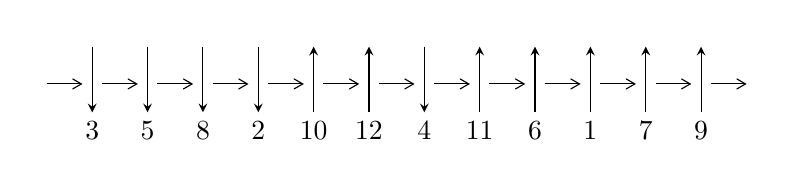
\begin{tikzpicture}[x=20pt, y=17pt]
	% nodes
	\node (C0) at (0, 0) {};
	\node (C1) at (1, 0) {};
	\node (C1U) at (1, +1) {};
	\node (C1D) at (1, -1) {3};

	\node (C2) at (2, 0) {};
	\node (C2U) at (2, +1) {};
	\node (C2D) at (2, -1) {5};

	\node (C3) at (3, 0) {};
	\node (C3U) at (3, +1) {};
	\node (C3D) at (3, -1) {8};

	\node (C4) at (4, 0) {};
	\node (C4U) at (4, +1) {};
	\node (C4D) at (4, -1) {2};

	\node (C5) at (5, 0) {};
	\node (C5U) at (5, +1) {};
	\node (C5D) at (5, -1) {10};

	\node (C6) at (6, 0) {};
	\node (C6U) at (6, +1) {};
	\node (C6D) at (6, -1) {12};

	\node (C7) at (7, 0) {};
	\node (C7U) at (7, +1) {};
	\node (C7D) at (7, -1) {4};

	\node (C8) at (8, 0) {};
	\node (C8U) at (8, +1) {};
	\node (C8D) at (8, -1) {11};

	\node (C9) at (9, 0) {};
	\node (C9U) at (9, +1) {};
	\node (C9D) at (9, -1) {6};

	\node (C10) at (10, 0) {};
	\node (C10U) at (10, +1) {};
	\node (C10D) at (10, -1) {1};

	\node (C11) at (11, 0) {};
	\node (C11U) at (11, +1) {};
	\node (C11D) at (11, -1) {7};

	\node (C12) at (12, 0) {};
	\node (C12U) at (12, +1) {};
	\node (C12D) at (12, -1) {9};
	\node (C13) at (13, 0) {};

	% arrows
	\draw[->,>={angle 60}]
	(C0) edge (C1) (C1) edge (C2) (C2) edge (C3) (C3) edge (C4) (C4) edge (C5) (C5) edge (C6) (C6) edge (C7) (C7) edge (C8) (C8) edge (C9) (C9) edge (C10) (C10) edge (C11) (C11) edge (C12) (C12) edge (C13) ;	\draw[->,>=stealth]
	(C1U) edge (C1D) (C2U) edge (C2D) (C3U) edge (C3D) (C4U) edge (C4D) (C5D) edge (C5U) (C6D) edge (C6U) (C7U) edge (C7D) (C8D) edge (C8U) (C9D) edge (C9U) (C10D) edge (C10U) (C11D) edge (C11U) (C12D) edge (C12U) ;
	\end{tikzpicture} \\
\hhline{~~} \\& 
\textbf{Solving Sequence} \\ \cline{2-2} 
 &
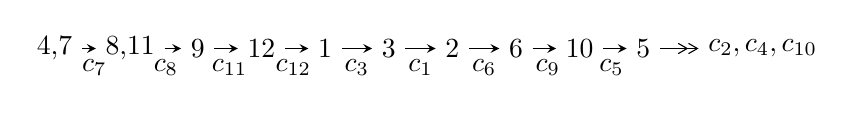
\begin{tikzpicture}[x=23pt, y=7pt]
	% node
	\node (A0) at (-1/8, 0) {4,7};
	\node (A1) at (17/16, 0) {8,11};
	\node (A2) at (17/8, 0) {9};
	\node (A3) at (25/8, 0) {12};
	\node (A4) at (33/8, 0) {1};
	\node (A5) at (41/8, 0) {3};
	\node (A6) at (49/8, 0) {2};
	\node (A7) at (57/8, 0) {6};
	\node (A8) at (65/8, 0) {10};
	\node (A9) at (73/8, 0) {5};
	\node (C1) at (1/2, -1) {$c_{7}$};
	\node (C2) at (13/8, -1) {$c_{8}$};
	\node (C3) at (21/8, -1) {$c_{11}$};
	\node (C4) at (29/8, -1) {$c_{12}$};
	\node (C5) at (37/8, -1) {$c_{3}$};
	\node (C6) at (45/8, -1) {$c_{1}$};
	\node (C7) at (53/8, -1) {$c_{6}$};
	\node (C8) at (61/8, -1) {$c_{9}$};
	\node (C9) at (69/8, -1) {$c_{5}$};
	\node (A10) at (11, 0) {$c_{2},c_{4},c_{10}$};

	% edge
	\draw[->,>=stealth]	
	(A0) edge (A1) (A1) edge (A2) (A2) edge (A3) (A3) edge (A4) (A4) edge (A5) (A5) edge (A6) (A6) edge (A7) (A7) edge (A8) (A8) edge (A9) ;
	\draw[->>,>={angle 60}]	
	(A9) edge (A10);
\end{tikzpicture} \\ 

\end{tabular} \\

\footnotetext{
The image of knot diagram is generated by the software ``\textbf{Draw programme}" developed by Andrew Bartholomew(\url{http://www.layer8.co.uk/maths/draw/index.htm\#Running-draw}), where we modified some parts for our purpose(\url{https://github.com/CATsTAILs/LinksPainter}).
}\phantom \\ \newline 
\centering \textbf{Ideals for irreducible components\footnotemark of $X_{\text{par}}$} 
 
\begin{align*}
I^u_{1}&=\langle 
1.87861\times10^{82} u^{47}+1.04155\times10^{83} u^{46}+\cdots+3.05135\times10^{83} b-3.51869\times10^{84},\\
\phantom{I^u_{1}}&\phantom{= \langle  }-3.38702\times10^{82} u^{47}-2.61769\times10^{83} u^{46}+\cdots+2.44108\times10^{84} a+1.57211\times10^{85},\\
\phantom{I^u_{1}}&\phantom{= \langle  }u^{48}+6 u^{47}+\cdots-608 u-128\rangle \\
I^u_{2}&=\langle 
34725 u^{16} a^3-26335 u^{16} a^2+\cdots-126824 a+31474,\;-2 u^{16} a^3+23 u^{16} a^2+\cdots+842 a+2659,\\
\phantom{I^u_{2}}&\phantom{= \langle  }u^{17}+2 u^{16}+\cdots-2 u-2\rangle \\
I^u_{3}&=\langle 
338183 u^{20}-78918 u^{19}+\cdots+334723 b+221323,\\
\phantom{I^u_{3}}&\phantom{= \langle  }-2123279 u^{20}+2034822 u^{19}+\cdots+334723 a+4096060,\;u^{21}- u^{20}+\cdots-2 u+1\rangle \\
I^u_{4}&=\langle 
-1746 a^5 u-3784 a^4 u+\cdots+44299 a-6066,\\
\phantom{I^u_{4}}&\phantom{= \langle  }a^6-4 a^5 u+4 a^5-10 a^4 u-6 a^4+18 a^3 u-27 a^3+33 a^2 u+3 a^2-27 a u+26 a+4 u-7,\;u^2- u+1\rangle \\
I^u_{5}&=\langle 
30 a^5 u-47 a^4 u+\cdots+104 a-142,\;a^6-4 a^5+4 a^4- a^3 u- a^3- a^2 u+5 a^2- a+2 u,\;u^2- u+1\rangle \\
\\
I^v_{1}&=\langle 
a,\;-8 v^2+b+26 v-7,\;4 v^3-14 v^2+7 v-1\rangle \\
I^v_{2}&=\langle 
a,\;b^4- b^3+2 b^2-2 b+1,\;v+1\rangle \\
\end{align*}
\raggedright * 7 irreducible components of $\dim_{\mathbb{C}}=0$, with total 168 representations.\\
\footnotetext{All coefficients of polynomials are rational numbers. But the coefficients are sometimes approximated in decimal forms when there is not enough margin.}
\newpage
\renewcommand{\arraystretch}{1}
\centering \section*{I. $I^u_{1}= \langle 1.88\times10^{82} u^{47}+1.04\times10^{83} u^{46}+\cdots+3.05\times10^{83} b-3.52\times10^{84},\;-3.39\times10^{82} u^{47}-2.62\times10^{83} u^{46}+\cdots+2.44\times10^{84} a+1.57\times10^{85},\;u^{48}+6 u^{47}+\cdots-608 u-128 \rangle$}
\flushleft \textbf{(i) Arc colorings}\\
\begin{tabular}{m{7pt} m{180pt} m{7pt} m{180pt} }
\flushright $a_{4}=$&$\begin{pmatrix}0\\u\end{pmatrix}$ \\
\flushright $a_{7}=$&$\begin{pmatrix}1\\0\end{pmatrix}$ \\
\flushright $a_{8}=$&$\begin{pmatrix}1\\u^2\end{pmatrix}$ \\
\flushright $a_{11}=$&$\begin{pmatrix}0.0138751 u^{47}+0.107235 u^{46}+\cdots-25.5601 u-6.44022\\-0.0615666 u^{47}-0.341342 u^{46}+\cdots+44.5324 u+11.5316\end{pmatrix}$ \\
\flushright $a_{9}=$&$\begin{pmatrix}0.0773618 u^{47}+0.445624 u^{46}+\cdots-51.2591 u-9.84291\\0.0862284 u^{47}+0.487720 u^{46}+\cdots-62.1112 u-12.9461\end{pmatrix}$ \\
\flushright $a_{12}=$&$\begin{pmatrix}-0.0476915 u^{47}-0.234107 u^{46}+\cdots+18.9724 u+5.09137\\-0.0615666 u^{47}-0.341342 u^{46}+\cdots+44.5324 u+11.5316\end{pmatrix}$ \\
\flushright $a_{1}=$&$\begin{pmatrix}-0.0708863 u^{47}-0.354435 u^{46}+\cdots+15.5178 u+0.0840131\\-0.109737 u^{47}-0.627104 u^{46}+\cdots+72.2764 u+12.8045\end{pmatrix}$ \\
\flushright $a_{3}=$&$\begin{pmatrix}u\\u^3+u\end{pmatrix}$ \\
\flushright $a_{2}=$&$\begin{pmatrix}-0.0947782 u^{47}-0.492160 u^{46}+\cdots+28.6120 u+2.50397\\-0.123753 u^{47}-0.710763 u^{46}+\cdots+85.7340 u+15.9448\end{pmatrix}$ \\
\flushright $a_{6}=$&$\begin{pmatrix}-0.116272 u^{47}-0.613951 u^{46}+\cdots+58.0413 u+11.2491\\-0.126215 u^{47}-0.696047 u^{46}+\cdots+77.0279 u+15.8185\end{pmatrix}$ \\
\flushright $a_{10}=$&$\begin{pmatrix}0.0714285 u^{47}+0.418715 u^{46}+\cdots-65.5831 u-16.3972\\0.123594 u^{47}+0.671965 u^{46}+\cdots-88.7374 u-22.0222\end{pmatrix}$ \\
\flushright $a_{5}=$&$\begin{pmatrix}0.0124958 u^{47}+0.0938805 u^{46}+\cdots-22.7356 u-3.64759\\0.0833820 u^{47}+0.448316 u^{46}+\cdots-38.2534 u-3.73160\end{pmatrix}$\\&\end{tabular}
\flushleft \textbf{(ii) Obstruction class $= -1$}\\~\\
\flushleft \textbf{(iii) Cusp Shapes $= -0.109672 u^{47}-0.524268 u^{46}+\cdots-20.2898 u-35.2434$}\\~\\
\newpage\renewcommand{\arraystretch}{1}
\flushleft \textbf{(iv) u-Polynomials at the component}\newline \\
\begin{tabular}{m{50pt}|m{274pt}}
Crossings & \hspace{64pt}u-Polynomials at each crossing \\
\hline $$\begin{aligned}c_{1}\end{aligned}$$&$\begin{aligned}
&u^{48}+25 u^{47}+\cdots+18800 u+256
\end{aligned}$\\
\hline $$\begin{aligned}c_{2},c_{4}\end{aligned}$$&$\begin{aligned}
&u^{48}-3 u^{47}+\cdots+76 u+16
\end{aligned}$\\
\hline $$\begin{aligned}c_{3},c_{7}\end{aligned}$$&$\begin{aligned}
&u^{48}+6 u^{47}+\cdots-608 u-128
\end{aligned}$\\
\hline $$\begin{aligned}c_{5},c_{6},c_{9}\\c_{11}\end{aligned}$$&$\begin{aligned}
&u^{48}+19 u^{46}+\cdots- u-1
\end{aligned}$\\
\hline $$\begin{aligned}c_{8},c_{10}\end{aligned}$$&$\begin{aligned}
&u^{48}-3 u^{47}+\cdots-23 u+1
\end{aligned}$\\
\hline $$\begin{aligned}c_{12}\end{aligned}$$&$\begin{aligned}
&u^{48}-51 u^{47}+\cdots-285212672 u+8388608
\end{aligned}$\\
\hline
\end{tabular}\\~\\
\newpage\renewcommand{\arraystretch}{1}
\flushleft \textbf{(v) Riley Polynomials at the component}\newline \\
\begin{tabular}{m{50pt}|m{274pt}}
Crossings & \hspace{64pt}Riley Polynomials at each crossing \\
\hline $$\begin{aligned}c_{1}\end{aligned}$$&$\begin{aligned}
&y^{48}- y^{47}+\cdots-279621376 y+65536
\end{aligned}$\\
\hline $$\begin{aligned}c_{2},c_{4}\end{aligned}$$&$\begin{aligned}
&y^{48}-25 y^{47}+\cdots-18800 y+256
\end{aligned}$\\
\hline $$\begin{aligned}c_{3},c_{7}\end{aligned}$$&$\begin{aligned}
&y^{48}+18 y^{47}+\cdots-158720 y+16384
\end{aligned}$\\
\hline $$\begin{aligned}c_{5},c_{6},c_{9}\\c_{11}\end{aligned}$$&$\begin{aligned}
&y^{48}+38 y^{47}+\cdots-31 y+1
\end{aligned}$\\
\hline $$\begin{aligned}c_{8},c_{10}\end{aligned}$$&$\begin{aligned}
&y^{48}+5 y^{47}+\cdots-237 y+1
\end{aligned}$\\
\hline $$\begin{aligned}c_{12}\end{aligned}$$&$\begin{aligned}
&y^{48}+5 y^{47}+\cdots-5875790138834944 y+70368744177664
\end{aligned}$\\
\hline
\end{tabular}\\~\\
\newpage\flushleft \textbf{(vi) Complex Volumes and Cusp Shapes}
$$\begin{array}{c|c|c}  
\text{Solutions to }I^u_{1}& \I (\text{vol} + \sqrt{-1}CS) & \text{Cusp shape}\\
 \hline 
\begin{aligned}
u &= \phantom{-}0.191047 + 1.007770 I \\
a &= \phantom{-}0.728739 + 0.164163 I \\
b &= -0.607742 - 0.383050 I\end{aligned}
 & \phantom{-}1.84375 + 0.90076 I & \phantom{-}5.50791 - 3.88202 I \\ \hline\begin{aligned}
u &= \phantom{-}0.191047 - 1.007770 I \\
a &= \phantom{-}0.728739 - 0.164163 I \\
b &= -0.607742 + 0.383050 I\end{aligned}
 & \phantom{-}1.84375 - 0.90076 I & \phantom{-}5.50791 + 3.88202 I \\ \hline\begin{aligned}
u &= -0.824028 + 0.494777 I \\
a &= \phantom{-}0.775855 - 0.447940 I \\
b &= -0.719486 - 0.096265 I\end{aligned}
 & -0.84172 - 2.79098 I & \phantom{-}2.56303 + 3.67085 I \\ \hline\begin{aligned}
u &= -0.824028 - 0.494777 I \\
a &= \phantom{-}0.775855 + 0.447940 I \\
b &= -0.719486 + 0.096265 I\end{aligned}
 & -0.84172 + 2.79098 I & \phantom{-}2.56303 - 3.67085 I \\ \hline\begin{aligned}
u &= -0.061009 + 1.092180 I \\
a &= -1.55932 + 0.14388 I \\
b &= \phantom{-}0.586610 + 0.474683 I\end{aligned}
 & \phantom{-}4.73028 - 1.19532 I & \phantom{-}7.39057 - 1.46823 I \\ \hline\begin{aligned}
u &= -0.061009 - 1.092180 I \\
a &= -1.55932 - 0.14388 I \\
b &= \phantom{-}0.586610 - 0.474683 I\end{aligned}
 & \phantom{-}4.73028 + 1.19532 I & \phantom{-}7.39057 + 1.46823 I \\ \hline\begin{aligned}
u &= \phantom{-}0.449465 + 1.031100 I \\
a &= -1.28963 - 0.62914 I \\
b &= \phantom{-}0.789520 + 0.202426 I\end{aligned}
 & \phantom{-}3.26311 - 3.26704 I & \phantom{-}7.67341 + 2.61304 I \\ \hline\begin{aligned}
u &= \phantom{-}0.449465 - 1.031100 I \\
a &= -1.28963 + 0.62914 I \\
b &= \phantom{-}0.789520 - 0.202426 I\end{aligned}
 & \phantom{-}3.26311 + 3.26704 I & \phantom{-}7.67341 - 2.61304 I \\ \hline\begin{aligned}
u &= \phantom{-}0.333088 + 1.109900 I \\
a &= -1.33371 - 0.49028 I \\
b &= \phantom{-}0.463573 - 0.639486 I\end{aligned}
 & \phantom{-}3.87618 - 3.65220 I & \phantom{-}3.08711 + 8.05406 I \\ \hline\begin{aligned}
u &= \phantom{-}0.333088 - 1.109900 I \\
a &= -1.33371 + 0.49028 I \\
b &= \phantom{-}0.463573 + 0.639486 I\end{aligned}
 & \phantom{-}3.87618 + 3.65220 I & \phantom{-}3.08711 - 8.05406 I\\
 \hline 
 \end{array}$$\newpage$$\begin{array}{c|c|c}  
\text{Solutions to }I^u_{1}& \I (\text{vol} + \sqrt{-1}CS) & \text{Cusp shape}\\
 \hline 
\begin{aligned}
u &= -0.538501 + 1.036350 I \\
a &= \phantom{-}0.711782 - 0.232849 I \\
b &= -0.803519 + 0.258105 I\end{aligned}
 & \phantom{-}0.15510 + 3.68398 I & \phantom{-}2.64964 - 1.96684 I \\ \hline\begin{aligned}
u &= -0.538501 - 1.036350 I \\
a &= \phantom{-}0.711782 + 0.232849 I \\
b &= -0.803519 - 0.258105 I\end{aligned}
 & \phantom{-}0.15510 - 3.68398 I & \phantom{-}2.64964 + 1.96684 I \\ \hline\begin{aligned}
u &= \phantom{-}1.066610 + 0.483181 I \\
a &= -0.048708 + 0.338357 I \\
b &= \phantom{-}0.44345 + 1.38767 I\end{aligned}
 & -7.17044 + 7.50868 I & -1.58512 - 3.77436 I \\ \hline\begin{aligned}
u &= \phantom{-}1.066610 - 0.483181 I \\
a &= -0.048708 - 0.338357 I \\
b &= \phantom{-}0.44345 - 1.38767 I\end{aligned}
 & -7.17044 - 7.50868 I & -1.58512 + 3.77436 I \\ \hline\begin{aligned}
u &= -0.593763 + 0.555003 I \\
a &= -0.050418 - 0.332210 I \\
b &= \phantom{-}0.32635 - 1.49374 I\end{aligned}
 & -11.74940 - 4.76001 I & -6.57262 - 2.96707 I \\ \hline\begin{aligned}
u &= -0.593763 - 0.555003 I \\
a &= -0.050418 + 0.332210 I \\
b &= \phantom{-}0.32635 + 1.49374 I\end{aligned}
 & -11.74940 + 4.76001 I & -6.57262 + 2.96707 I \\ \hline\begin{aligned}
u &= -0.601845 + 1.052800 I \\
a &= \phantom{-}2.05390 + 0.10513 I \\
b &= -0.46620 - 1.43355 I\end{aligned}
 & -10.21060 + 9.59449 I & -3.60142 - 6.18831 I \\ \hline\begin{aligned}
u &= -0.601845 - 1.052800 I \\
a &= \phantom{-}2.05390 - 0.10513 I \\
b &= -0.46620 + 1.43355 I\end{aligned}
 & -10.21060 - 9.59449 I & -3.60142 + 6.18831 I \\ \hline\begin{aligned}
u &= -0.485413 + 0.601421 I \\
a &= -1.28070 + 1.69925 I \\
b &= \phantom{-}0.627305 - 0.012830 I\end{aligned}
 & -1.262120 + 0.607533 I & \phantom{-}3.19613 - 5.27342 I \\ \hline\begin{aligned}
u &= -0.485413 - 0.601421 I \\
a &= -1.28070 - 1.69925 I \\
b &= \phantom{-}0.627305 + 0.012830 I\end{aligned}
 & -1.262120 - 0.607533 I & \phantom{-}3.19613 + 5.27342 I\\
 \hline 
 \end{array}$$\newpage$$\begin{array}{c|c|c}  
\text{Solutions to }I^u_{1}& \I (\text{vol} + \sqrt{-1}CS) & \text{Cusp shape}\\
 \hline 
\begin{aligned}
u &= -0.635379 + 1.085340 I \\
a &= -1.035040 + 0.645312 I \\
b &= \phantom{-}0.890242 - 0.142272 I\end{aligned}
 & \phantom{-}0.95191 + 8.23122 I & \phantom{-}3.50123 - 7.17855 I \\ \hline\begin{aligned}
u &= -0.635379 - 1.085340 I \\
a &= -1.035040 - 0.645312 I \\
b &= \phantom{-}0.890242 + 0.142272 I\end{aligned}
 & \phantom{-}0.95191 - 8.23122 I & \phantom{-}3.50123 + 7.17855 I \\ \hline\begin{aligned}
u &= -1.096040 + 0.664816 I \\
a &= -0.054336 - 0.338178 I \\
b &= \phantom{-}0.49492 - 1.44926 I\end{aligned}
 & -9.5879 - 12.5892 I & -3.60578 + 7.24500 I \\ \hline\begin{aligned}
u &= -1.096040 - 0.664816 I \\
a &= -0.054336 + 0.338178 I \\
b &= \phantom{-}0.49492 + 1.44926 I\end{aligned}
 & -9.5879 + 12.5892 I & -3.60578 - 7.24500 I \\ \hline\begin{aligned}
u &= \phantom{-}0.638998 + 0.071034 I \\
a &= \phantom{-}1.28773 - 1.29641 I \\
b &= -0.345569 - 0.223570 I\end{aligned}
 & \phantom{-}0.673431 + 0.110718 I & \phantom{-}7.7390 - 14.7279 I \\ \hline\begin{aligned}
u &= \phantom{-}0.638998 - 0.071034 I \\
a &= \phantom{-}1.28773 + 1.29641 I \\
b &= -0.345569 + 0.223570 I\end{aligned}
 & \phantom{-}0.673431 - 0.110718 I & \phantom{-}7.7390 + 14.7279 I \\ \hline\begin{aligned}
u &= \phantom{-}0.710349 + 1.174450 I \\
a &= \phantom{-}1.68838 + 0.12583 I \\
b &= -0.53527 + 1.45440 I\end{aligned}
 & -4.9700 - 13.8549 I & \phantom{-0.000000 } 0 \\ \hline\begin{aligned}
u &= \phantom{-}0.710349 - 1.174450 I \\
a &= \phantom{-}1.68838 - 0.12583 I \\
b &= -0.53527 - 1.45440 I\end{aligned}
 & -4.9700 + 13.8549 I & \phantom{-0.000000 } 0 \\ \hline\begin{aligned}
u &= -0.420346 + 0.423788 I \\
a &= -0.053647 + 0.334365 I \\
b &= \phantom{-}0.17258 + 1.45355 I\end{aligned}
 & -11.27470 + 5.48110 I & -7.3979 - 14.4496 I \\ \hline\begin{aligned}
u &= -0.420346 - 0.423788 I \\
a &= -0.053647 - 0.334365 I \\
b &= \phantom{-}0.17258 - 1.45355 I\end{aligned}
 & -11.27470 - 5.48110 I & -7.3979 + 14.4496 I\\
 \hline 
 \end{array}$$\newpage$$\begin{array}{c|c|c}  
\text{Solutions to }I^u_{1}& \I (\text{vol} + \sqrt{-1}CS) & \text{Cusp shape}\\
 \hline 
\begin{aligned}
u &= -0.806830 + 1.155070 I \\
a &= \phantom{-}1.66382 - 0.32906 I \\
b &= -0.54117 - 1.49832 I\end{aligned}
 & -7.9747 + 19.4545 I & \phantom{-0.000000 } 0 \\ \hline\begin{aligned}
u &= -0.806830 - 1.155070 I \\
a &= \phantom{-}1.66382 + 0.32906 I \\
b &= -0.54117 + 1.49832 I\end{aligned}
 & -7.9747 - 19.4545 I & \phantom{-0.000000 } 0 \\ \hline\begin{aligned}
u &= \phantom{-}0.33726 + 1.38273 I \\
a &= \phantom{-}1.048030 - 0.444775 I \\
b &= -0.535063 + 1.197840 I\end{aligned}
 & -0.00671 - 10.39530 I & \phantom{-0.000000 } 0 \\ \hline\begin{aligned}
u &= \phantom{-}0.33726 - 1.38273 I \\
a &= \phantom{-}1.048030 + 0.444775 I \\
b &= -0.535063 - 1.197840 I\end{aligned}
 & -0.00671 + 10.39530 I & \phantom{-0.000000 } 0 \\ \hline\begin{aligned}
u &= -0.22239 + 1.42242 I \\
a &= \phantom{-}0.721683 + 0.463533 I \\
b &= -0.458297 - 1.049830 I\end{aligned}
 & \phantom{-}1.00442 + 4.31512 I & \phantom{-0.000000 } 0 \\ \hline\begin{aligned}
u &= -0.22239 - 1.42242 I \\
a &= \phantom{-}0.721683 - 0.463533 I \\
b &= -0.458297 + 1.049830 I\end{aligned}
 & \phantom{-}1.00442 - 4.31512 I & \phantom{-0.000000 } 0 \\ \hline\begin{aligned}
u &= -0.89457 + 1.16056 I \\
a &= -1.001830 + 0.221515 I \\
b &= \phantom{-}0.118376 + 1.224700 I\end{aligned}
 & -5.81153 + 10.03740 I & \phantom{-0.000000 } 0 \\ \hline\begin{aligned}
u &= -0.89457 - 1.16056 I \\
a &= -1.001830 - 0.221515 I \\
b &= \phantom{-}0.118376 - 1.224700 I\end{aligned}
 & -5.81153 - 10.03740 I & \phantom{-0.000000 } 0 \\ \hline\begin{aligned}
u &= \phantom{-}1.47382 + 0.09648 I \\
a &= -0.023063 - 0.280597 I \\
b &= \phantom{-}0.214306 - 1.129300 I\end{aligned}
 & -5.30932 - 4.33878 I & \phantom{-0.000000 } 0 \\ \hline\begin{aligned}
u &= \phantom{-}1.47382 - 0.09648 I \\
a &= -0.023063 + 0.280597 I \\
b &= \phantom{-}0.214306 + 1.129300 I\end{aligned}
 & -5.30932 + 4.33878 I & \phantom{-0.000000 } 0\\
 \hline 
 \end{array}$$\newpage$$\begin{array}{c|c|c}  
\text{Solutions to }I^u_{1}& \I (\text{vol} + \sqrt{-1}CS) & \text{Cusp shape}\\
 \hline 
\begin{aligned}
u &= \phantom{-}0.90750 + 1.20267 I \\
a &= -0.791351 - 0.168123 I \\
b &= \phantom{-}0.072284 - 1.150090 I\end{aligned}
 & -2.35143 - 4.21639 I & \phantom{-0.000000 } 0 \\ \hline\begin{aligned}
u &= \phantom{-}0.90750 - 1.20267 I \\
a &= -0.791351 + 0.168123 I \\
b &= \phantom{-}0.072284 + 1.150090 I\end{aligned}
 & -2.35143 + 4.21639 I & \phantom{-0.000000 } 0 \\ \hline\begin{aligned}
u &= -0.441911\phantom{ +0.000000I} \\
a &= \phantom{-}1.53998\phantom{ +0.000000I} \\
b &= \phantom{-}0.237250\phantom{ +0.000000I}\end{aligned}
 & -1.26980\phantom{ +0.000000I} & -9.92780\phantom{ +0.000000I} \\ \hline\begin{aligned}
u &= -1.32729 + 0.82837 I \\
a &= -0.162773 + 0.297503 I \\
b &= \phantom{-}0.006720 + 1.165660 I\end{aligned}
 & -7.13142 - 2.34962 I & \phantom{-0.000000 } 0 \\ \hline\begin{aligned}
u &= -1.32729 - 0.82837 I \\
a &= -0.162773 - 0.297503 I \\
b &= \phantom{-}0.006720 - 1.165660 I\end{aligned}
 & -7.13142 + 2.34962 I & \phantom{-0.000000 } 0 \\ \hline\begin{aligned}
u &= -0.55430 + 1.47189 I \\
a &= -0.471137 - 0.489578 I \\
b &= -0.089207 + 1.159830 I\end{aligned}
 & -7.97723 - 1.25475 I & \phantom{-0.000000 } 0 \\ \hline\begin{aligned}
u &= -0.55430 - 1.47189 I \\
a &= -0.471137 + 0.489578 I \\
b &= -0.089207 - 1.159830 I\end{aligned}
 & -7.97723 + 1.25475 I & \phantom{-0.000000 } 0 \\ \hline\begin{aligned}
u &= \phantom{-}0.349047\phantom{ +0.000000I} \\
a &= \phantom{-}1.28651\phantom{ +0.000000I} \\
b &= -0.446661\phantom{ +0.000000I}\end{aligned}
 & \phantom{-}0.908064\phantom{ +0.000000I} & \phantom{-}11.6320\phantom{ +0.000000I}\\
 \hline 
 \end{array}$$\newpage\newpage\renewcommand{\arraystretch}{1}
\centering \section*{II. $I^u_{2}= \langle 3.47\times10^{4} a^{3} u^{16}-2.63\times10^{4} a^{2} u^{16}+\cdots-1.27\times10^{5} a+3.15\times10^{4},\;-2 u^{16} a^3+23 u^{16} a^2+\cdots+842 a+2659,\;u^{17}+2 u^{16}+\cdots-2 u-2 \rangle$}
\flushleft \textbf{(i) Arc colorings}\\
\begin{tabular}{m{7pt} m{180pt} m{7pt} m{180pt} }
\flushright $a_{4}=$&$\begin{pmatrix}0\\u\end{pmatrix}$ \\
\flushright $a_{7}=$&$\begin{pmatrix}1\\0\end{pmatrix}$ \\
\flushright $a_{8}=$&$\begin{pmatrix}1\\u^2\end{pmatrix}$ \\
\flushright $a_{11}=$&$\begin{pmatrix}a\\-1.15889 a^{3} u^{16}+0.878888 a^{2} u^{16}+\cdots+4.23255 a-1.05039\end{pmatrix}$ \\
\flushright $a_{9}=$&$\begin{pmatrix}0.454445 a^{3} u^{16}-0.378888 a^{2} u^{16}+\cdots-1.44961 a+3.55039\\-0.295555 a^{2} u^{16}-0.352223 u^{16}+\cdots+0.565879 a^{2}+1.21706\end{pmatrix}$ \\
\flushright $a_{12}=$&$\begin{pmatrix}-1.15889 a^{3} u^{16}+0.878888 a^{2} u^{16}+\cdots+5.23255 a-1.05039\\-1.15889 a^{3} u^{16}+0.878888 a^{2} u^{16}+\cdots+4.23255 a-1.05039\end{pmatrix}$ \\
\flushright $a_{1}=$&$\begin{pmatrix}-\frac{1}{2} u^{16}-\frac{1}{4} u^{15}+\cdots-\frac{1}{2} u-\frac{1}{2}\\-\frac{1}{2} u^{16}-\frac{1}{2} u^{15}+\cdots-\frac{3}{4} u^2+\frac{1}{2}\end{pmatrix}$ \\
\flushright $a_{3}=$&$\begin{pmatrix}u\\u^3+u\end{pmatrix}$ \\
\flushright $a_{2}=$&$\begin{pmatrix}-\frac{1}{4} u^{16}-\frac{3}{4} u^{14}+\cdots-\frac{3}{2} u-\frac{1}{2}\\-\frac{1}{4} u^{16}-\frac{1}{2} u^{14}+\cdots-\frac{1}{2} u^2- u\end{pmatrix}$ \\
\flushright $a_{6}=$&$\begin{pmatrix}-0.811107 a^{3} u^{16}+1.06778 a^{2} u^{16}+\cdots+0.418636 a-4.13176\\-0.356661 a^{3} u^{16}+0.688893 a^{2} u^{16}+\cdots-1.03097 a-2.58136\end{pmatrix}$ \\
\flushright $a_{10}=$&$\begin{pmatrix}0.908891 a^{3} u^{16}-0.795555 a^{2} u^{16}+\cdots+1.93412 a-1.28294\\0.158891 a^{3} u^{16}-0.212221 a^{2} u^{16}+\cdots+4.10079 a-0.616273\end{pmatrix}$ \\
\flushright $a_{5}=$&$\begin{pmatrix}-\frac{1}{2} u^{16}- u^{15}+\cdots-\frac{11}{4} u^2+\frac{1}{2}\\-\frac{3}{4} u^{15}-\frac{3}{4} u^{14}+\cdots+\frac{1}{2} u+1\end{pmatrix}$\\&\end{tabular}
\flushleft \textbf{(ii) Obstruction class $= -1$}\\~\\
\flushleft \textbf{(iii) Cusp Shapes $= -\frac{12718}{7491} u^{16} a^3+\frac{4539}{2497} u^{16} a^2+\cdots+\frac{82924}{7491} a-\frac{17808}{2497}$}\\~\\
\newpage\renewcommand{\arraystretch}{1}
\flushleft \textbf{(iv) u-Polynomials at the component}\newline \\
\begin{tabular}{m{50pt}|m{274pt}}
Crossings & \hspace{64pt}u-Polynomials at each crossing \\
\hline $$\begin{aligned}c_{1}\end{aligned}$$&$\begin{aligned}
&(u^{17}+8 u^{16}+\cdots+3 u+1)^{4}
\end{aligned}$\\
\hline $$\begin{aligned}c_{2},c_{4}\end{aligned}$$&$\begin{aligned}
&(u^{17}-2 u^{16}+\cdots- u+1)^{4}
\end{aligned}$\\
\hline $$\begin{aligned}c_{3},c_{7}\end{aligned}$$&$\begin{aligned}
&(u^{17}+2 u^{16}+\cdots-2 u-2)^{4}
\end{aligned}$\\
\hline $$\begin{aligned}c_{5},c_{6},c_{9}\\c_{11}\end{aligned}$$&$\begin{aligned}
&u^{68}-2 u^{67}+\cdots+942 u+61
\end{aligned}$\\
\hline $$\begin{aligned}c_{8},c_{10}\end{aligned}$$&$\begin{aligned}
&u^{68}+18 u^{67}+\cdots+8600 u+373
\end{aligned}$\\
\hline $$\begin{aligned}c_{12}\end{aligned}$$&$\begin{aligned}
&(u^2+u+1)^{34}
\end{aligned}$\\
\hline
\end{tabular}\\~\\
\newpage\renewcommand{\arraystretch}{1}
\flushleft \textbf{(v) Riley Polynomials at the component}\newline \\
\begin{tabular}{m{50pt}|m{274pt}}
Crossings & \hspace{64pt}Riley Polynomials at each crossing \\
\hline $$\begin{aligned}c_{1}\end{aligned}$$&$\begin{aligned}
&(y^{17}+4 y^{16}+\cdots-13 y-1)^{4}
\end{aligned}$\\
\hline $$\begin{aligned}c_{2},c_{4}\end{aligned}$$&$\begin{aligned}
&(y^{17}-8 y^{16}+\cdots+3 y-1)^{4}
\end{aligned}$\\
\hline $$\begin{aligned}c_{3},c_{7}\end{aligned}$$&$\begin{aligned}
&(y^{17}+6 y^{16}+\cdots+8 y-4)^{4}
\end{aligned}$\\
\hline $$\begin{aligned}c_{5},c_{6},c_{9}\\c_{11}\end{aligned}$$&$\begin{aligned}
&y^{68}+54 y^{67}+\cdots+221616 y+3721
\end{aligned}$\\
\hline $$\begin{aligned}c_{8},c_{10}\end{aligned}$$&$\begin{aligned}
&y^{68}+14 y^{67}+\cdots+20523884 y+139129
\end{aligned}$\\
\hline $$\begin{aligned}c_{12}\end{aligned}$$&$\begin{aligned}
&(y^2+y+1)^{34}
\end{aligned}$\\
\hline
\end{tabular}\\~\\
\newpage\flushleft \textbf{(vi) Complex Volumes and Cusp Shapes}
$$\begin{array}{c|c|c}  
\text{Solutions to }I^u_{2}& \I (\text{vol} + \sqrt{-1}CS) & \text{Cusp shape}\\
 \hline 
\begin{aligned}
u &= -0.742615 + 0.650908 I \\
a &= -0.858913 - 0.213402 I \\
b &= -0.66649 + 1.56071 I\end{aligned}
 & -8.59404 - 3.25712 I & -8.14847 + 4.31915 I \\ \hline\begin{aligned}
u &= -0.742615 + 0.650908 I \\
a &= -0.17250 - 1.68551 I \\
b &= -0.040339 - 1.225610 I\end{aligned}
 & -8.59404 + 0.80264 I & -8.14847 - 2.60905 I \\ \hline\begin{aligned}
u &= -0.742615 + 0.650908 I \\
a &= -2.43226 + 1.27156 I \\
b &= \phantom{-}0.59407 + 1.60818 I\end{aligned}
 & -8.59404 + 0.80264 I & -8.14847 - 2.60905 I \\ \hline\begin{aligned}
u &= -0.742615 + 0.650908 I \\
a &= \phantom{-}2.51978 - 1.83542 I \\
b &= \phantom{-}0.058310 - 1.272450 I\end{aligned}
 & -8.59404 - 3.25712 I & -8.14847 + 4.31915 I \\ \hline\begin{aligned}
u &= -0.742615 - 0.650908 I \\
a &= -0.858913 + 0.213402 I \\
b &= -0.66649 - 1.56071 I\end{aligned}
 & -8.59404 + 3.25712 I & -8.14847 - 4.31915 I \\ \hline\begin{aligned}
u &= -0.742615 - 0.650908 I \\
a &= -0.17250 + 1.68551 I \\
b &= -0.040339 + 1.225610 I\end{aligned}
 & -8.59404 - 0.80264 I & -8.14847 + 2.60905 I \\ \hline\begin{aligned}
u &= -0.742615 - 0.650908 I \\
a &= -2.43226 - 1.27156 I \\
b &= \phantom{-}0.59407 - 1.60818 I\end{aligned}
 & -8.59404 - 0.80264 I & -8.14847 + 2.60905 I \\ \hline\begin{aligned}
u &= -0.742615 - 0.650908 I \\
a &= \phantom{-}2.51978 + 1.83542 I \\
b &= \phantom{-}0.058310 + 1.272450 I\end{aligned}
 & -8.59404 + 3.25712 I & -8.14847 - 4.31915 I \\ \hline\begin{aligned}
u &= -0.834865 + 0.265014 I \\
a &= -0.016132 + 0.733452 I \\
b &= \phantom{-}0.960620 - 0.161520 I\end{aligned}
 & -2.31524 - 2.46376 I & \phantom{-}0.56834 + 2.58870 I \\ \hline\begin{aligned}
u &= -0.834865 + 0.265014 I \\
a &= \phantom{-}0.284668 - 0.665934 I \\
b &= \phantom{-}0.509050 - 0.033729 I\end{aligned}
 & -2.31524 + 1.59601 I & \phantom{-}0.56834 - 4.33950 I\\
 \hline 
 \end{array}$$\newpage$$\begin{array}{c|c|c}  
\text{Solutions to }I^u_{2}& \I (\text{vol} + \sqrt{-1}CS) & \text{Cusp shape}\\
 \hline 
\begin{aligned}
u &= -0.834865 + 0.265014 I \\
a &= \phantom{-}0.475849 + 0.326477 I \\
b &= -0.232899 + 1.178170 I\end{aligned}
 & -2.31524 - 2.46376 I & \phantom{-}0.56834 + 2.58870 I \\ \hline\begin{aligned}
u &= -0.834865 + 0.265014 I \\
a &= \phantom{-}0.403399 - 0.262157 I \\
b &= \phantom{-}0.007533 - 1.104820 I\end{aligned}
 & -2.31524 + 1.59601 I & \phantom{-}0.56834 - 4.33950 I \\ \hline\begin{aligned}
u &= -0.834865 - 0.265014 I \\
a &= -0.016132 - 0.733452 I \\
b &= \phantom{-}0.960620 + 0.161520 I\end{aligned}
 & -2.31524 + 2.46376 I & \phantom{-}0.56834 - 2.58870 I \\ \hline\begin{aligned}
u &= -0.834865 - 0.265014 I \\
a &= \phantom{-}0.284668 + 0.665934 I \\
b &= \phantom{-}0.509050 + 0.033729 I\end{aligned}
 & -2.31524 - 1.59601 I & \phantom{-}0.56834 + 4.33950 I \\ \hline\begin{aligned}
u &= -0.834865 - 0.265014 I \\
a &= \phantom{-}0.475849 - 0.326477 I \\
b &= -0.232899 - 1.178170 I\end{aligned}
 & -2.31524 + 2.46376 I & \phantom{-}0.56834 - 2.58870 I \\ \hline\begin{aligned}
u &= -0.834865 - 0.265014 I \\
a &= \phantom{-}0.403399 + 0.262157 I \\
b &= \phantom{-}0.007533 + 1.104820 I\end{aligned}
 & -2.31524 - 1.59601 I & \phantom{-}0.56834 + 4.33950 I \\ \hline\begin{aligned}
u &= \phantom{-}0.976738 + 0.562668 I \\
a &= \phantom{-}0.453582 + 0.523609 I \\
b &= \phantom{-}0.097566 + 0.148491 I\end{aligned}
 & -4.32437 + 2.61783 I & -2.43915 - 0.65285 I \\ \hline\begin{aligned}
u &= \phantom{-}0.976738 + 0.562668 I \\
a &= -0.163065 - 0.655845 I \\
b &= \phantom{-}1.225180 + 0.226983 I\end{aligned}
 & -4.32437 + 6.67759 I & -2.43915 - 7.58105 I \\ \hline\begin{aligned}
u &= \phantom{-}0.976738 + 0.562668 I \\
a &= \phantom{-}0.462635 - 0.371400 I \\
b &= -0.336705 - 1.223300 I\end{aligned}
 & -4.32437 + 6.67759 I & -2.43915 - 7.58105 I \\ \hline\begin{aligned}
u &= \phantom{-}0.976738 + 0.562668 I \\
a &= \phantom{-}0.286253 + 0.249449 I \\
b &= \phantom{-}0.321037 + 1.119110 I\end{aligned}
 & -4.32437 + 2.61783 I & -2.43915 - 0.65285 I\\
 \hline 
 \end{array}$$\newpage$$\begin{array}{c|c|c}  
\text{Solutions to }I^u_{2}& \I (\text{vol} + \sqrt{-1}CS) & \text{Cusp shape}\\
 \hline 
\begin{aligned}
u &= \phantom{-}0.976738 - 0.562668 I \\
a &= \phantom{-}0.453582 - 0.523609 I \\
b &= \phantom{-}0.097566 - 0.148491 I\end{aligned}
 & -4.32437 - 2.61783 I & -2.43915 + 0.65285 I \\ \hline\begin{aligned}
u &= \phantom{-}0.976738 - 0.562668 I \\
a &= -0.163065 + 0.655845 I \\
b &= \phantom{-}1.225180 - 0.226983 I\end{aligned}
 & -4.32437 - 6.67759 I & -2.43915 + 7.58105 I \\ \hline\begin{aligned}
u &= \phantom{-}0.976738 - 0.562668 I \\
a &= \phantom{-}0.462635 + 0.371400 I \\
b &= -0.336705 + 1.223300 I\end{aligned}
 & -4.32437 - 6.67759 I & -2.43915 + 7.58105 I \\ \hline\begin{aligned}
u &= \phantom{-}0.976738 - 0.562668 I \\
a &= \phantom{-}0.286253 - 0.249449 I \\
b &= \phantom{-}0.321037 - 1.119110 I\end{aligned}
 & -4.32437 - 2.61783 I & -2.43915 + 0.65285 I \\ \hline\begin{aligned}
u &= -0.003992 + 0.842342 I \\
a &= \phantom{-}0.823514 + 0.703163 I \\
b &= -0.188923 + 1.380570 I\end{aligned}
 & -3.62498 - 3.49944 I & \phantom{-}1.63583 + 8.12938 I \\ \hline\begin{aligned}
u &= -0.003992 + 0.842342 I \\
a &= \phantom{-}0.354576 + 0.342592 I \\
b &= -0.17222 - 1.57777 I\end{aligned}
 & -3.62498 + 0.56033 I & \phantom{-}1.63583 + 1.20118 I \\ \hline\begin{aligned}
u &= -0.003992 + 0.842342 I \\
a &= -1.14706 + 1.36568 I \\
b &= \phantom{-}0.865544 - 1.043820 I\end{aligned}
 & -3.62498 - 3.49944 I & \phantom{-}1.63583 + 8.12938 I \\ \hline\begin{aligned}
u &= -0.003992 + 0.842342 I \\
a &= \phantom{-}1.59887 - 1.09681 I \\
b &= \phantom{-}0.125548 + 0.823426 I\end{aligned}
 & -3.62498 + 0.56033 I & \phantom{-}1.63583 + 1.20118 I \\ \hline\begin{aligned}
u &= -0.003992 - 0.842342 I \\
a &= \phantom{-}0.823514 - 0.703163 I \\
b &= -0.188923 - 1.380570 I\end{aligned}
 & -3.62498 + 3.49944 I & \phantom{-}1.63583 - 8.12938 I \\ \hline\begin{aligned}
u &= -0.003992 - 0.842342 I \\
a &= \phantom{-}0.354576 - 0.342592 I \\
b &= -0.17222 + 1.57777 I\end{aligned}
 & -3.62498 - 0.56033 I & \phantom{-}1.63583 - 1.20118 I\\
 \hline 
 \end{array}$$\newpage$$\begin{array}{c|c|c}  
\text{Solutions to }I^u_{2}& \I (\text{vol} + \sqrt{-1}CS) & \text{Cusp shape}\\
 \hline 
\begin{aligned}
u &= -0.003992 - 0.842342 I \\
a &= -1.14706 - 1.36568 I \\
b &= \phantom{-}0.865544 + 1.043820 I\end{aligned}
 & -3.62498 + 3.49944 I & \phantom{-}1.63583 - 8.12938 I \\ \hline\begin{aligned}
u &= -0.003992 - 0.842342 I \\
a &= \phantom{-}1.59887 + 1.09681 I \\
b &= \phantom{-}0.125548 - 0.823426 I\end{aligned}
 & -3.62498 - 0.56033 I & \phantom{-}1.63583 - 1.20118 I \\ \hline\begin{aligned}
u &= -0.656745 + 1.004700 I \\
a &= \phantom{-}0.146155 - 1.227280 I \\
b &= -0.025709 - 1.355530 I\end{aligned}
 & -7.51458 + 8.60052 I & -5.26005 - 9.89862 I \\ \hline\begin{aligned}
u &= -0.656745 + 1.004700 I \\
a &= -0.376762 - 0.223958 I \\
b &= -0.55941 + 1.77505 I\end{aligned}
 & -7.51458 + 4.54075 I & -5.26005 - 2.97041 I \\ \hline\begin{aligned}
u &= -0.656745 + 1.004700 I \\
a &= -1.80331 + 0.32050 I \\
b &= \phantom{-}0.84173 + 1.60733 I\end{aligned}
 & -7.51458 + 8.60052 I & -5.26005 - 9.89862 I \\ \hline\begin{aligned}
u &= -0.656745 + 1.004700 I \\
a &= \phantom{-}1.99063 - 0.75779 I \\
b &= -0.066671 - 1.194250 I\end{aligned}
 & -7.51458 + 4.54075 I & -5.26005 - 2.97041 I \\ \hline\begin{aligned}
u &= -0.656745 - 1.004700 I \\
a &= \phantom{-}0.146155 + 1.227280 I \\
b &= -0.025709 + 1.355530 I\end{aligned}
 & -7.51458 - 8.60052 I & -5.26005 + 9.89862 I \\ \hline\begin{aligned}
u &= -0.656745 - 1.004700 I \\
a &= -0.376762 + 0.223958 I \\
b &= -0.55941 - 1.77505 I\end{aligned}
 & -7.51458 - 4.54075 I & -5.26005 + 2.97041 I \\ \hline\begin{aligned}
u &= -0.656745 - 1.004700 I \\
a &= -1.80331 - 0.32050 I \\
b &= \phantom{-}0.84173 - 1.60733 I\end{aligned}
 & -7.51458 - 8.60052 I & -5.26005 + 9.89862 I \\ \hline\begin{aligned}
u &= -0.656745 - 1.004700 I \\
a &= \phantom{-}1.99063 + 0.75779 I \\
b &= -0.066671 + 1.194250 I\end{aligned}
 & -7.51458 - 4.54075 I & -5.26005 + 2.97041 I\\
 \hline 
 \end{array}$$\newpage$$\begin{array}{c|c|c}  
\text{Solutions to }I^u_{2}& \I (\text{vol} + \sqrt{-1}CS) & \text{Cusp shape}\\
 \hline 
\begin{aligned}
u &= -0.110097 + 1.246510 I \\
a &= -0.537569 + 0.828636 I \\
b &= \phantom{-}0.247183 - 0.880435 I\end{aligned}
 & \phantom{-}3.09988 + 0.68177 I & \phantom{-}3.84242 + 0.32700 I \\ \hline\begin{aligned}
u &= -0.110097 + 1.246510 I \\
a &= \phantom{-}1.147850 - 0.201747 I \\
b &= -0.922464 - 0.394135 I\end{aligned}
 & \phantom{-}3.09988 + 0.68177 I & \phantom{-}3.84242 + 0.32700 I \\ \hline\begin{aligned}
u &= -0.110097 + 1.246510 I \\
a &= \phantom{-}1.301120 + 0.007909 I \\
b &= -1.089750 + 0.222504 I\end{aligned}
 & \phantom{-}3.09988 + 4.74154 I & \phantom{-}3.84242 - 6.60120 I \\ \hline\begin{aligned}
u &= -0.110097 + 1.246510 I \\
a &= -1.063350 - 0.849870 I \\
b &= \phantom{-}0.323575 + 0.999592 I\end{aligned}
 & \phantom{-}3.09988 + 4.74154 I & \phantom{-}3.84242 - 6.60120 I \\ \hline\begin{aligned}
u &= -0.110097 - 1.246510 I \\
a &= -0.537569 - 0.828636 I \\
b &= \phantom{-}0.247183 + 0.880435 I\end{aligned}
 & \phantom{-}3.09988 - 0.68177 I & \phantom{-}3.84242 - 0.32700 I \\ \hline\begin{aligned}
u &= -0.110097 - 1.246510 I \\
a &= \phantom{-}1.147850 + 0.201747 I \\
b &= -0.922464 + 0.394135 I\end{aligned}
 & \phantom{-}3.09988 - 0.68177 I & \phantom{-}3.84242 - 0.32700 I \\ \hline\begin{aligned}
u &= -0.110097 - 1.246510 I \\
a &= \phantom{-}1.301120 - 0.007909 I \\
b &= -1.089750 - 0.222504 I\end{aligned}
 & \phantom{-}3.09988 - 4.74154 I & \phantom{-}3.84242 + 6.60120 I \\ \hline\begin{aligned}
u &= -0.110097 - 1.246510 I \\
a &= -1.063350 + 0.849870 I \\
b &= \phantom{-}0.323575 - 0.999592 I\end{aligned}
 & \phantom{-}3.09988 - 4.74154 I & \phantom{-}3.84242 + 6.60120 I \\ \hline\begin{aligned}
u &= -0.578864 + 1.116300 I \\
a &= \phantom{-}1.204300 - 0.022501 I \\
b &= -0.488361 - 1.049000 I\end{aligned}
 & \phantom{-}0.11501 + 3.48170 I & \phantom{-}2.25126 - 0.38080 I \\ \hline\begin{aligned}
u &= -0.578864 + 1.116300 I \\
a &= \phantom{-}1.27173 - 0.65139 I \\
b &= -1.312600 - 0.151182 I\end{aligned}
 & \phantom{-}0.11501 + 7.54146 I & \phantom{-}2.25126 - 7.30900 I\\
 \hline 
 \end{array}$$\newpage$$\begin{array}{c|c|c}  
\text{Solutions to }I^u_{2}& \I (\text{vol} + \sqrt{-1}CS) & \text{Cusp shape}\\
 \hline 
\begin{aligned}
u &= -0.578864 + 1.116300 I \\
a &= -0.194398 - 0.198117 I \\
b &= \phantom{-}0.042359 - 0.283882 I\end{aligned}
 & \phantom{-}0.11501 + 3.48170 I & \phantom{-}2.25126 - 0.38080 I \\ \hline\begin{aligned}
u &= -0.578864 + 1.116300 I \\
a &= -1.96774 - 0.11289 I \\
b &= \phantom{-}0.381291 + 1.203870 I\end{aligned}
 & \phantom{-}0.11501 + 7.54146 I & \phantom{-}2.25126 - 7.30900 I \\ \hline\begin{aligned}
u &= -0.578864 - 1.116300 I \\
a &= \phantom{-}1.204300 + 0.022501 I \\
b &= -0.488361 + 1.049000 I\end{aligned}
 & \phantom{-}0.11501 - 3.48170 I & \phantom{-}2.25126 + 0.38080 I \\ \hline\begin{aligned}
u &= -0.578864 - 1.116300 I \\
a &= \phantom{-}1.27173 + 0.65139 I \\
b &= -1.312600 + 0.151182 I\end{aligned}
 & \phantom{-}0.11501 - 7.54146 I & \phantom{-}2.25126 + 7.30900 I \\ \hline\begin{aligned}
u &= -0.578864 - 1.116300 I \\
a &= -0.194398 + 0.198117 I \\
b &= \phantom{-}0.042359 + 0.283882 I\end{aligned}
 & \phantom{-}0.11501 - 3.48170 I & \phantom{-}2.25126 + 0.38080 I \\ \hline\begin{aligned}
u &= -0.578864 - 1.116300 I \\
a &= -1.96774 + 0.11289 I \\
b &= \phantom{-}0.381291 - 1.203870 I\end{aligned}
 & \phantom{-}0.11501 - 7.54146 I & \phantom{-}2.25126 + 7.30900 I \\ \hline\begin{aligned}
u &= \phantom{-}0.718492 + 1.129370 I \\
a &= \phantom{-}1.275350 + 0.228864 I \\
b &= -0.553021 + 1.205800 I\end{aligned}
 & -2.53156 - 8.80385 I & -1.10622 + 3.94851 I \\ \hline\begin{aligned}
u &= \phantom{-}0.718492 + 1.129370 I \\
a &= \phantom{-}1.097970 + 0.736493 I \\
b &= -1.40257 + 0.22167 I\end{aligned}
 & -2.53156 - 12.86360 I & -1.10622 + 10.87671 I \\ \hline\begin{aligned}
u &= \phantom{-}0.718492 + 1.129370 I \\
a &= -0.420731 + 0.192335 I \\
b &= \phantom{-}0.164364 + 0.168623 I\end{aligned}
 & -2.53156 - 8.80385 I & -1.10622 + 3.94851 I \\ \hline\begin{aligned}
u &= \phantom{-}0.718492 + 1.129370 I \\
a &= -1.89005 - 0.20697 I \\
b &= \phantom{-}0.406612 - 1.245470 I\end{aligned}
 & -2.53156 - 12.86360 I & -1.10622 + 10.87671 I\\
 \hline 
 \end{array}$$\newpage$$\begin{array}{c|c|c}  
\text{Solutions to }I^u_{2}& \I (\text{vol} + \sqrt{-1}CS) & \text{Cusp shape}\\
 \hline 
\begin{aligned}
u &= \phantom{-}0.718492 - 1.129370 I \\
a &= \phantom{-}1.275350 - 0.228864 I \\
b &= -0.553021 - 1.205800 I\end{aligned}
 & -2.53156 + 8.80385 I & -1.10622 - 3.94851 I \\ \hline\begin{aligned}
u &= \phantom{-}0.718492 - 1.129370 I \\
a &= \phantom{-}1.097970 - 0.736493 I \\
b &= -1.40257 - 0.22167 I\end{aligned}
 & -2.53156 + 12.86360 I & -1.10622 - 10.87671 I \\ \hline\begin{aligned}
u &= \phantom{-}0.718492 - 1.129370 I \\
a &= -0.420731 - 0.192335 I \\
b &= \phantom{-}0.164364 - 0.168623 I\end{aligned}
 & -2.53156 + 8.80385 I & -1.10622 - 3.94851 I \\ \hline\begin{aligned}
u &= \phantom{-}0.718492 - 1.129370 I \\
a &= -1.89005 + 0.20697 I \\
b &= \phantom{-}0.406612 + 1.245470 I\end{aligned}
 & -2.53156 + 12.86360 I & -1.10622 - 10.87671 I \\ \hline\begin{aligned}
u &= \phantom{-}0.463897\phantom{ +0.000000I} \\
a &= -4.47126 + 2.76907 I \\
b &= -0.397720 + 1.155250 I\end{aligned}
 & -6.19292 - 2.02988 I & -10.68792 + 3.46410 I \\ \hline\begin{aligned}
u &= \phantom{-}0.463897\phantom{ +0.000000I} \\
a &= -4.47126 - 2.76907 I \\
b &= -0.397720 - 1.155250 I\end{aligned}
 & -6.19292 + 2.02988 I & -10.68792 - 3.46410 I \\ \hline\begin{aligned}
u &= \phantom{-}0.463897\phantom{ +0.000000I} \\
a &= -0.58311 + 11.52350 I \\
b &= \phantom{-}0.284280 + 1.351730 I\end{aligned}
 & -6.19292 + 2.02988 I & -10.68792 - 3.46410 I \\ \hline\begin{aligned}
u &= \phantom{-}0.463897\phantom{ +0.000000I} \\
a &= -0.58311 - 11.52350 I \\
b &= \phantom{-}0.284280 - 1.351730 I\end{aligned}
 & -6.19292 - 2.02988 I & -10.68792 + 3.46410 I\\
 \hline 
 \end{array}$$\newpage\newpage\renewcommand{\arraystretch}{1}
\centering \section*{III. $I^u_{3}= \langle 3.38\times10^{5} u^{20}-7.89\times10^{4} u^{19}+\cdots+3.35\times10^{5} b+2.21\times10^{5},\;-2.12\times10^{6} u^{20}+2.03\times10^{6} u^{19}+\cdots+3.35\times10^{5} a+4.10\times10^{6},\;u^{21}- u^{20}+\cdots-2 u+1 \rangle$}
\flushleft \textbf{(i) Arc colorings}\\
\begin{tabular}{m{7pt} m{180pt} m{7pt} m{180pt} }
\flushright $a_{4}=$&$\begin{pmatrix}0\\u\end{pmatrix}$ \\
\flushright $a_{7}=$&$\begin{pmatrix}1\\0\end{pmatrix}$ \\
\flushright $a_{8}=$&$\begin{pmatrix}1\\u^2\end{pmatrix}$ \\
\flushright $a_{11}=$&$\begin{pmatrix}6.34339 u^{20}-6.07912 u^{19}+\cdots+17.6956 u-12.2372\\-1.01034 u^{20}+0.235771 u^{19}+\cdots-2.20402 u-0.661212\end{pmatrix}$ \\
\flushright $a_{9}=$&$\begin{pmatrix}0.312375 u^{20}+2.96012 u^{19}+\cdots+3.86554 u+11.9528\\1.35474 u^{20}-1.24479 u^{19}+\cdots+3.63887 u-1.82860\end{pmatrix}$ \\
\flushright $a_{12}=$&$\begin{pmatrix}5.33305 u^{20}-5.84335 u^{19}+\cdots+15.4916 u-12.8984\\-1.01034 u^{20}+0.235771 u^{19}+\cdots-2.20402 u-0.661212\end{pmatrix}$ \\
\flushright $a_{1}=$&$\begin{pmatrix}-1.24963 u^{20}+0.461943 u^{19}+\cdots-4.25896 u+0.00811417\\-0.0988130 u^{20}+0.262465 u^{19}+\cdots+0.213051 u+0.0131213\end{pmatrix}$ \\
\flushright $a_{3}=$&$\begin{pmatrix}u\\u^3+u\end{pmatrix}$ \\
\flushright $a_{2}=$&$\begin{pmatrix}-1.47255 u^{20}+1.20487 u^{19}+\cdots-4.89251 u+0.996355\\-0.180295 u^{20}+0.767210 u^{19}+\cdots+0.842431 u+0.481356\end{pmatrix}$ \\
\flushright $a_{6}=$&$\begin{pmatrix}4.42387 u^{20}-1.98590 u^{19}+\cdots+22.5450 u+0.373646\\-0.411406 u^{20}+0.417725 u^{19}+\cdots-3.61084 u-0.603057\end{pmatrix}$ \\
\flushright $a_{10}=$&$\begin{pmatrix}4.98866 u^{20}-4.83433 u^{19}+\cdots+14.0567 u-9.40856\\-1.01034 u^{20}+0.235771 u^{19}+\cdots-2.20402 u-0.661212\end{pmatrix}$ \\
\flushright $a_{5}=$&$\begin{pmatrix}1.34293 u^{20}-0.354687 u^{19}+\cdots+4.79776 u-0.782680\\0.0932980 u^{20}+0.107256 u^{19}+\cdots+0.538795 u-0.774566\end{pmatrix}$\\&\end{tabular}
\flushleft \textbf{(ii) Obstruction class $= 1$}\\~\\
\flushleft \textbf{(iii) Cusp Shapes $= \frac{2811940}{334723} u^{20}-\frac{1365409}{334723} u^{19}+\cdots+\frac{14890533}{334723} u-\frac{3065752}{334723}$}\\~\\
\newpage\renewcommand{\arraystretch}{1}
\flushleft \textbf{(iv) u-Polynomials at the component}\newline \\
\begin{tabular}{m{50pt}|m{274pt}}
Crossings & \hspace{64pt}u-Polynomials at each crossing \\
\hline $$\begin{aligned}c_{1}\end{aligned}$$&$\begin{aligned}
&u^{21}-11 u^{20}+\cdots+2 u-1
\end{aligned}$\\
\hline $$\begin{aligned}c_{2}\end{aligned}$$&$\begin{aligned}
&u^{21}+3 u^{20}+\cdots-4 u-1
\end{aligned}$\\
\hline $$\begin{aligned}c_{3}\end{aligned}$$&$\begin{aligned}
&u^{21}+u^{20}+\cdots-2 u-1
\end{aligned}$\\
\hline $$\begin{aligned}c_{4}\end{aligned}$$&$\begin{aligned}
&u^{21}-3 u^{20}+\cdots-4 u+1
\end{aligned}$\\
\hline $$\begin{aligned}c_{5},c_{11}\end{aligned}$$&$\begin{aligned}
&u^{21}+12 u^{19}+\cdots+5 u-1
\end{aligned}$\\
\hline $$\begin{aligned}c_{6},c_{9}\end{aligned}$$&$\begin{aligned}
&u^{21}+12 u^{19}+\cdots+5 u+1
\end{aligned}$\\
\hline $$\begin{aligned}c_{7}\end{aligned}$$&$\begin{aligned}
&u^{21}- u^{20}+\cdots-2 u+1
\end{aligned}$\\
\hline $$\begin{aligned}c_{8},c_{10}\end{aligned}$$&$\begin{aligned}
&u^{21}-3 u^{20}+\cdots-3 u+1
\end{aligned}$\\
\hline $$\begin{aligned}c_{12}\end{aligned}$$&$\begin{aligned}
&u^{21}+3 u^{20}+\cdots-3 u-1
\end{aligned}$\\
\hline
\end{tabular}\\~\\
\newpage\renewcommand{\arraystretch}{1}
\flushleft \textbf{(v) Riley Polynomials at the component}\newline \\
\begin{tabular}{m{50pt}|m{274pt}}
Crossings & \hspace{64pt}Riley Polynomials at each crossing \\
\hline $$\begin{aligned}c_{1}\end{aligned}$$&$\begin{aligned}
&y^{21}+y^{20}+\cdots-6 y-1
\end{aligned}$\\
\hline $$\begin{aligned}c_{2},c_{4}\end{aligned}$$&$\begin{aligned}
&y^{21}-11 y^{20}+\cdots+2 y-1
\end{aligned}$\\
\hline $$\begin{aligned}c_{3},c_{7}\end{aligned}$$&$\begin{aligned}
&y^{21}+9 y^{20}+\cdots-6 y-1
\end{aligned}$\\
\hline $$\begin{aligned}c_{5},c_{6},c_{9}\\c_{11}\end{aligned}$$&$\begin{aligned}
&y^{21}+24 y^{20}+\cdots+99 y-1
\end{aligned}$\\
\hline $$\begin{aligned}c_{8},c_{10}\end{aligned}$$&$\begin{aligned}
&y^{21}+3 y^{20}+\cdots-3 y-1
\end{aligned}$\\
\hline $$\begin{aligned}c_{12}\end{aligned}$$&$\begin{aligned}
&y^{21}+3 y^{20}+\cdots-3 y-1
\end{aligned}$\\
\hline
\end{tabular}\\~\\
\newpage\flushleft \textbf{(vi) Complex Volumes and Cusp Shapes}
$$\begin{array}{c|c|c}  
\text{Solutions to }I^u_{3}& \I (\text{vol} + \sqrt{-1}CS) & \text{Cusp shape}\\
 \hline 
\begin{aligned}
u &= \phantom{-}0.490243 + 0.937388 I \\
a &= \phantom{-}0.514333 + 0.625527 I \\
b &= -0.528540 - 1.286100 I\end{aligned}
 & -5.52103 - 1.78110 I & -3.65173 + 3.65315 I \\ \hline\begin{aligned}
u &= \phantom{-}0.490243 - 0.937388 I \\
a &= \phantom{-}0.514333 - 0.625527 I \\
b &= -0.528540 + 1.286100 I\end{aligned}
 & -5.52103 + 1.78110 I & -3.65173 - 3.65315 I \\ \hline\begin{aligned}
u &= -0.156277 + 1.122180 I \\
a &= -1.217350 + 0.179026 I \\
b &= \phantom{-}0.410410 + 0.113082 I\end{aligned}
 & \phantom{-}4.06250 + 2.43837 I & \phantom{-}5.17498 - 3.14519 I \\ \hline\begin{aligned}
u &= -0.156277 - 1.122180 I \\
a &= -1.217350 - 0.179026 I \\
b &= \phantom{-}0.410410 - 0.113082 I\end{aligned}
 & \phantom{-}4.06250 - 2.43837 I & \phantom{-}5.17498 + 3.14519 I \\ \hline\begin{aligned}
u &= -0.130234 + 0.829741 I \\
a &= \phantom{-}1.35637 - 0.71728 I \\
b &= -0.43014 + 1.34934 I\end{aligned}
 & -3.93501 - 2.17155 I & \phantom{-}0.14652 + 1.48581 I \\ \hline\begin{aligned}
u &= -0.130234 - 0.829741 I \\
a &= \phantom{-}1.35637 + 0.71728 I \\
b &= -0.43014 - 1.34934 I\end{aligned}
 & -3.93501 + 2.17155 I & \phantom{-}0.14652 - 1.48581 I \\ \hline\begin{aligned}
u &= -0.659203 + 0.963090 I \\
a &= \phantom{-}1.009120 - 0.683478 I \\
b &= -0.18280 - 1.48861 I\end{aligned}
 & -7.11068 + 6.86906 I & -4.04608 - 5.76368 I \\ \hline\begin{aligned}
u &= -0.659203 - 0.963090 I \\
a &= \phantom{-}1.009120 + 0.683478 I \\
b &= -0.18280 + 1.48861 I\end{aligned}
 & -7.11068 - 6.86906 I & -4.04608 + 5.76368 I \\ \hline\begin{aligned}
u &= \phantom{-}0.410688 + 0.721803 I \\
a &= \phantom{-}1.56660 + 0.92039 I \\
b &= -0.280481 + 1.376890 I\end{aligned}
 & -4.50106 - 2.68972 I & \phantom{-}0.55053 + 1.78075 I \\ \hline\begin{aligned}
u &= \phantom{-}0.410688 - 0.721803 I \\
a &= \phantom{-}1.56660 - 0.92039 I \\
b &= -0.280481 - 1.376890 I\end{aligned}
 & -4.50106 + 2.68972 I & \phantom{-}0.55053 - 1.78075 I\\
 \hline 
 \end{array}$$\newpage$$\begin{array}{c|c|c}  
\text{Solutions to }I^u_{3}& \I (\text{vol} + \sqrt{-1}CS) & \text{Cusp shape}\\
 \hline 
\begin{aligned}
u &= \phantom{-}1.156740 + 0.305908 I \\
a &= -0.338936 - 0.137814 I \\
b &= -0.304972 - 1.054660 I\end{aligned}
 & -5.35947 + 3.69430 I & -6.58451 - 3.53350 I \\ \hline\begin{aligned}
u &= \phantom{-}1.156740 - 0.305908 I \\
a &= -0.338936 + 0.137814 I \\
b &= -0.304972 + 1.054660 I\end{aligned}
 & -5.35947 - 3.69430 I & -6.58451 + 3.53350 I \\ \hline\begin{aligned}
u &= -0.730687 + 0.973520 I \\
a &= \phantom{-}1.040580 - 0.020751 I \\
b &= \phantom{-}0.089617 - 1.248120 I\end{aligned}
 & -7.52481 - 1.55740 I & -4.73995 + 2.30181 I \\ \hline\begin{aligned}
u &= -0.730687 - 0.973520 I \\
a &= \phantom{-}1.040580 + 0.020751 I \\
b &= \phantom{-}0.089617 + 1.248120 I\end{aligned}
 & -7.52481 + 1.55740 I & -4.73995 - 2.30181 I \\ \hline\begin{aligned}
u &= \phantom{-}0.731610 + 1.181440 I \\
a &= -1.096200 - 0.010581 I \\
b &= \phantom{-}0.526976 - 0.918183 I\end{aligned}
 & -2.90296 - 10.25050 I & -2.57335 + 9.34499 I \\ \hline\begin{aligned}
u &= \phantom{-}0.731610 - 1.181440 I \\
a &= -1.096200 + 0.010581 I \\
b &= \phantom{-}0.526976 + 0.918183 I\end{aligned}
 & -2.90296 + 10.25050 I & -2.57335 - 9.34499 I \\ \hline\begin{aligned}
u &= -0.640346 + 1.260900 I \\
a &= -0.845339 - 0.135710 I \\
b &= \phantom{-}0.381374 + 0.865230 I\end{aligned}
 & -0.24350 + 4.56805 I & -0.64289 - 8.18526 I \\ \hline\begin{aligned}
u &= -0.640346 - 1.260900 I \\
a &= -0.845339 + 0.135710 I \\
b &= \phantom{-}0.381374 - 0.865230 I\end{aligned}
 & -0.24350 - 4.56805 I & -0.64289 + 8.18526 I \\ \hline\begin{aligned}
u &= -0.549197\phantom{ +0.000000I} \\
a &= \phantom{-}3.01565\phantom{ +0.000000I} \\
b &= -0.100536\phantom{ +0.000000I}\end{aligned}
 & \phantom{-}0.498833\phantom{ +0.000000I} & -32.6110\phantom{ +0.000000I} \\ \hline\begin{aligned}
u &= \phantom{-}0.302066 + 0.377168 I \\
a &= -8.99701 + 2.20814 I \\
b &= \phantom{-}0.368826 - 1.244610 I\end{aligned}
 & -6.69180 - 1.84270 I & -6.8280 + 14.0564 I\\
 \hline 
 \end{array}$$\newpage$$\begin{array}{c|c|c}  
\text{Solutions to }I^u_{3}& \I (\text{vol} + \sqrt{-1}CS) & \text{Cusp shape}\\
 \hline 
\begin{aligned}
u &= \phantom{-}0.302066 - 0.377168 I \\
a &= -8.99701 - 2.20814 I \\
b &= \phantom{-}0.368826 + 1.244610 I\end{aligned}
 & -6.69180 + 1.84270 I & -6.8280 - 14.0564 I\\
 \hline 
 \end{array}$$\newpage\newpage\renewcommand{\arraystretch}{1}
\centering \section*{IV. $I^u_{4}= \langle -1746 a^5 u-3784 a^4 u+\cdots+44299 a-6066,\;-4 a^5 u-10 a^4 u+\cdots+26 a-7,\;u^2- u+1 \rangle$}
\flushleft \textbf{(i) Arc colorings}\\
\begin{tabular}{m{7pt} m{180pt} m{7pt} m{180pt} }
\flushright $a_{4}=$&$\begin{pmatrix}0\\u\end{pmatrix}$ \\
\flushright $a_{7}=$&$\begin{pmatrix}1\\0\end{pmatrix}$ \\
\flushright $a_{8}=$&$\begin{pmatrix}1\\u-1\end{pmatrix}$ \\
\flushright $a_{11}=$&$\begin{pmatrix}a\\0.232583 a^{5} u+0.504063 a^{4} u+\cdots-5.90103 a+0.808046\end{pmatrix}$ \\
\flushright $a_{9}=$&$\begin{pmatrix}-0.285067 a^{5} u-0.983216 a^{4} u+\cdots+4.04822 a+0.452911\\-0.273611 a^{5} u-0.980152 a^{4} u+\cdots+4.54909 a+0.472093\end{pmatrix}$ \\
\flushright $a_{12}=$&$\begin{pmatrix}0.232583 a^{5} u+0.504063 a^{4} u+\cdots-4.90103 a+0.808046\\0.232583 a^{5} u+0.504063 a^{4} u+\cdots-5.90103 a+0.808046\end{pmatrix}$ \\
\flushright $a_{1}=$&$\begin{pmatrix}-0.0166511 a^{5} u+0.332756 a^{4} u+\cdots-1.12335 a+0.344212\\0.0410284 a^{5} u+0.476089 a^{4} u+\cdots-0.648062 a+0.719861\end{pmatrix}$ \\
\flushright $a_{3}=$&$\begin{pmatrix}u\\u-1\end{pmatrix}$ \\
\flushright $a_{2}=$&$\begin{pmatrix}0.136806 a^{5} u+0.490076 a^{4} u+\cdots-2.27454 a+1.76395\\0.189290 a^{5} u+0.969229 a^{4} u+\cdots-2.42174 a+2.50300\end{pmatrix}$ \\
\flushright $a_{6}=$&$\begin{pmatrix}0.309445 a^{5} u+1.79206 a^{4} u+\cdots-4.81964 a-1.38884\\0.0243772 a^{5} u+0.808845 a^{4} u+\cdots-0.771413 a-2.93593\end{pmatrix}$ \\
\flushright $a_{10}=$&$\begin{pmatrix}-0.131877 a^{5} u-0.244572 a^{4} u+\cdots+2.58306 a+0.686160\\-0.0492873 a^{5} u-0.455042 a^{4} u+\cdots-1.08512 a+1.49887\end{pmatrix}$ \\
\flushright $a_{5}=$&$\begin{pmatrix}-0.148262 a^{5} u-0.493140 a^{4} u+\cdots+1.77368 a-1.78314\\-0.131610 a^{5} u-0.825896 a^{4} u+\cdots+2.89703 a-2.12735\end{pmatrix}$\\&\end{tabular}
\flushleft \textbf{(ii) Obstruction class $= -1$}\\~\\
\flushleft \textbf{(iii) Cusp Shapes $= 8 u-6$}\\~\\
\newpage\renewcommand{\arraystretch}{1}
\flushleft \textbf{(iv) u-Polynomials at the component}\newline \\
\begin{tabular}{m{50pt}|m{274pt}}
Crossings & \hspace{64pt}u-Polynomials at each crossing \\
\hline $$\begin{aligned}c_{1}\end{aligned}$$&$\begin{aligned}
&(u^6+4 u^5+6 u^4+3 u^3- u^2- u+1)^2
\end{aligned}$\\
\hline $$\begin{aligned}c_{2},c_{4}\end{aligned}$$&$\begin{aligned}
&(u^6-2 u^4+u^3+u^2- u+1)^2
\end{aligned}$\\
\hline $$\begin{aligned}c_{3},c_{7}\end{aligned}$$&$\begin{aligned}
&(u^2- u+1)^6
\end{aligned}$\\
\hline $$\begin{aligned}c_{5},c_{6},c_{9}\\c_{11}\end{aligned}$$&$\begin{aligned}
&u^{12}+6 u^{10}+\cdots-2 u+4
\end{aligned}$\\
\hline $$\begin{aligned}c_{8},c_{10}\end{aligned}$$&$\begin{aligned}
&u^{12}+4 u^{11}+\cdots+14 u+13
\end{aligned}$\\
\hline $$\begin{aligned}c_{12}\end{aligned}$$&$\begin{aligned}
&(u^2+u+1)^6
\end{aligned}$\\
\hline
\end{tabular}\\~\\
\newpage\renewcommand{\arraystretch}{1}
\flushleft \textbf{(v) Riley Polynomials at the component}\newline \\
\begin{tabular}{m{50pt}|m{274pt}}
Crossings & \hspace{64pt}Riley Polynomials at each crossing \\
\hline $$\begin{aligned}c_{1}\end{aligned}$$&$\begin{aligned}
&(y^6-4 y^5+10 y^4-11 y^3+19 y^2-3 y+1)^2
\end{aligned}$\\
\hline $$\begin{aligned}c_{2},c_{4}\end{aligned}$$&$\begin{aligned}
&(y^6-4 y^5+6 y^4-3 y^3- y^2+y+1)^2
\end{aligned}$\\
\hline $$\begin{aligned}c_{3},c_{7},c_{12}\end{aligned}$$&$\begin{aligned}
&(y^2+y+1)^6
\end{aligned}$\\
\hline $$\begin{aligned}c_{5},c_{6},c_{9}\\c_{11}\end{aligned}$$&$\begin{aligned}
&y^{12}+12 y^{11}+\cdots+228 y+16
\end{aligned}$\\
\hline $$\begin{aligned}c_{8},c_{10}\end{aligned}$$&$\begin{aligned}
&y^{12}+8 y^{11}+\cdots+558 y+169
\end{aligned}$\\
\hline
\end{tabular}\\~\\
\newpage\flushleft \textbf{(vi) Complex Volumes and Cusp Shapes}
$$\begin{array}{c|c|c}  
\text{Solutions to }I^u_{4}& \I (\text{vol} + \sqrt{-1}CS) & \text{Cusp shape}\\
 \hline 
\begin{aligned}
u &= \phantom{-}0.500000 + 0.866025 I \\
a &= \phantom{-}0.800900 + 0.692255 I \\
b &= \phantom{-}0.020130 - 0.405138 I\end{aligned}
 & -4.93480 - 4.05977 I & -2.00000 + 6.92820 I \\ \hline\begin{aligned}
u &= \phantom{-}0.500000 + 0.866025 I \\
a &= \phantom{-}0.37705 + 1.39893 I \\
b &= -0.086959 + 1.331210 I\end{aligned}
 & -4.93480 - 4.05977 I & -2.00000 + 6.92820 I \\ \hline\begin{aligned}
u &= \phantom{-}0.500000 + 0.866025 I \\
a &= \phantom{-}0.296620 + 0.036933 I \\
b &= \phantom{-}0.12517 + 1.51446 I\end{aligned}
 & -4.93480 - 4.05977 I & -2.00000 + 6.92820 I \\ \hline\begin{aligned}
u &= \phantom{-}0.500000 + 0.866025 I \\
a &= \phantom{-}1.72107 + 0.97581 I \\
b &= -1.127070 + 0.261490 I\end{aligned}
 & -4.93480 - 4.05977 I & -2.00000 + 6.92820 I \\ \hline\begin{aligned}
u &= \phantom{-}0.500000 + 0.866025 I \\
a &= -2.29509 + 0.00735 I \\
b &= \phantom{-}0.77338 - 1.47468 I\end{aligned}
 & -4.93480 - 4.05977 I & -2.00000 + 6.92820 I \\ \hline\begin{aligned}
u &= \phantom{-}0.500000 + 0.866025 I \\
a &= -2.90055 + 0.35282 I \\
b &= \phantom{-}0.295351 - 1.227340 I\end{aligned}
 & -4.93480 - 4.05977 I & -2.00000 + 6.92820 I \\ \hline\begin{aligned}
u &= \phantom{-}0.500000 - 0.866025 I \\
a &= \phantom{-}0.800900 - 0.692255 I \\
b &= \phantom{-}0.020130 + 0.405138 I\end{aligned}
 & -4.93480 + 4.05977 I & -2.00000 - 6.92820 I \\ \hline\begin{aligned}
u &= \phantom{-}0.500000 - 0.866025 I \\
a &= \phantom{-}0.37705 - 1.39893 I \\
b &= -0.086959 - 1.331210 I\end{aligned}
 & -4.93480 + 4.05977 I & -2.00000 - 6.92820 I \\ \hline\begin{aligned}
u &= \phantom{-}0.500000 - 0.866025 I \\
a &= \phantom{-}0.296620 - 0.036933 I \\
b &= \phantom{-}0.12517 - 1.51446 I\end{aligned}
 & -4.93480 + 4.05977 I & -2.00000 - 6.92820 I \\ \hline\begin{aligned}
u &= \phantom{-}0.500000 - 0.866025 I \\
a &= \phantom{-}1.72107 - 0.97581 I \\
b &= -1.127070 - 0.261490 I\end{aligned}
 & -4.93480 + 4.05977 I & -2.00000 - 6.92820 I\\
 \hline 
 \end{array}$$\newpage$$\begin{array}{c|c|c}  
\text{Solutions to }I^u_{4}& \I (\text{vol} + \sqrt{-1}CS) & \text{Cusp shape}\\
 \hline 
\begin{aligned}
u &= \phantom{-}0.500000 - 0.866025 I \\
a &= -2.29509 - 0.00735 I \\
b &= \phantom{-}0.77338 + 1.47468 I\end{aligned}
 & -4.93480 + 4.05977 I & -2.00000 - 6.92820 I \\ \hline\begin{aligned}
u &= \phantom{-}0.500000 - 0.866025 I \\
a &= -2.90055 - 0.35282 I \\
b &= \phantom{-}0.295351 + 1.227340 I\end{aligned}
 & -4.93480 + 4.05977 I & -2.00000 - 6.92820 I\\
 \hline 
 \end{array}$$\newpage\newpage\renewcommand{\arraystretch}{1}
\centering \section*{V. $I^u_{5}= \langle 30 a^5 u-47 a^4 u+\cdots+104 a-142,\;- a^3 u- a^2 u+\cdots+5 a^2- a,\;u^2- u+1 \rangle$}
\flushleft \textbf{(i) Arc colorings}\\
\begin{tabular}{m{7pt} m{180pt} m{7pt} m{180pt} }
\flushright $a_{4}=$&$\begin{pmatrix}0\\u\end{pmatrix}$ \\
\flushright $a_{7}=$&$\begin{pmatrix}1\\0\end{pmatrix}$ \\
\flushright $a_{8}=$&$\begin{pmatrix}1\\u-1\end{pmatrix}$ \\
\flushright $a_{11}=$&$\begin{pmatrix}a\\-0.189873 a^{5} u+0.297468 a^{4} u+\cdots-0.658228 a+0.898734\end{pmatrix}$ \\
\flushright $a_{9}=$&$\begin{pmatrix}0.462025 a^{5} u-1.74051 a^{4} u+\cdots-1.03165 a+1.37975\\0.0506329 a^{5} u-0.0126582 a^{4} u+\cdots+0.708861 a+1.49367\end{pmatrix}$ \\
\flushright $a_{12}=$&$\begin{pmatrix}-0.189873 a^{5} u+0.297468 a^{4} u+\cdots+0.341772 a+0.898734\\-0.189873 a^{5} u+0.297468 a^{4} u+\cdots-0.658228 a+0.898734\end{pmatrix}$ \\
\flushright $a_{1}=$&$\begin{pmatrix}-0.101266 a^{5} u+0.0253165 a^{4} u+\cdots-1.41772 a+1.01266\\0.0253165 a^{5} u-0.00632911 a^{4} u+\cdots-0.645570 a+0.746835\end{pmatrix}$ \\
\flushright $a_{3}=$&$\begin{pmatrix}u\\u-1\end{pmatrix}$ \\
\flushright $a_{2}=$&$\begin{pmatrix}-0.0822785 a^{5} u+0.145570 a^{4} u+\cdots+0.348101 a+0.822785\\0.481013 a^{5} u-1.62025 a^{4} u+\cdots-0.265823 a+1.18987\end{pmatrix}$ \\
\flushright $a_{6}=$&$\begin{pmatrix}-0.139241 a^{5} u+0.284810 a^{4} u+\cdots+1.05063 a-1.60759\\0.322785 a^{5} u-1.45570 a^{4} u+\cdots+0.0189873 a-2.22785\end{pmatrix}$ \\
\flushright $a_{10}=$&$\begin{pmatrix}0.151899 a^{5} u-1.03797 a^{4} u+\cdots-0.873418 a+0.481013\\-0.354430 a^{5} u+1.08861 a^{4} u+\cdots-1.96203 a+1.54430\end{pmatrix}$ \\
\flushright $a_{5}=$&$\begin{pmatrix}-0.455696 a^{5} u+1.61392 a^{4} u+\cdots-0.379747 a-0.443038\\-0.354430 a^{5} u+1.58861 a^{4} u+\cdots+1.03797 a-1.45570\end{pmatrix}$\\&\end{tabular}
\flushleft \textbf{(ii) Obstruction class $= -1$}\\~\\
\flushleft \textbf{(iii) Cusp Shapes $= -2$}\\~\\
\newpage\renewcommand{\arraystretch}{1}
\flushleft \textbf{(iv) u-Polynomials at the component}\newline \\
\begin{tabular}{m{50pt}|m{274pt}}
Crossings & \hspace{64pt}u-Polynomials at each crossing \\
\hline $$\begin{aligned}c_{1}\end{aligned}$$&$\begin{aligned}
&(u^6+4 u^5+6 u^4+3 u^3- u^2- u+1)^2
\end{aligned}$\\
\hline $$\begin{aligned}c_{2},c_{4}\end{aligned}$$&$\begin{aligned}
&(u^6-2 u^4+u^3+u^2- u+1)^2
\end{aligned}$\\
\hline $$\begin{aligned}c_{3},c_{7}\end{aligned}$$&$\begin{aligned}
&(u^2- u+1)^6
\end{aligned}$\\
\hline $$\begin{aligned}c_{5},c_{6},c_{9}\\c_{11}\end{aligned}$$&$\begin{aligned}
&u^{12}+6 u^{10}+\cdots-8 u+1
\end{aligned}$\\
\hline $$\begin{aligned}c_{8},c_{10}\end{aligned}$$&$\begin{aligned}
&u^{12}+4 u^{11}+\cdots+14 u+4
\end{aligned}$\\
\hline $$\begin{aligned}c_{12}\end{aligned}$$&$\begin{aligned}
&(u^2+u+1)^6
\end{aligned}$\\
\hline
\end{tabular}\\~\\
\newpage\renewcommand{\arraystretch}{1}
\flushleft \textbf{(v) Riley Polynomials at the component}\newline \\
\begin{tabular}{m{50pt}|m{274pt}}
Crossings & \hspace{64pt}Riley Polynomials at each crossing \\
\hline $$\begin{aligned}c_{1}\end{aligned}$$&$\begin{aligned}
&(y^6-4 y^5+10 y^4-11 y^3+19 y^2-3 y+1)^2
\end{aligned}$\\
\hline $$\begin{aligned}c_{2},c_{4}\end{aligned}$$&$\begin{aligned}
&(y^6-4 y^5+6 y^4-3 y^3- y^2+y+1)^2
\end{aligned}$\\
\hline $$\begin{aligned}c_{3},c_{7},c_{12}\end{aligned}$$&$\begin{aligned}
&(y^2+y+1)^6
\end{aligned}$\\
\hline $$\begin{aligned}c_{5},c_{6},c_{9}\\c_{11}\end{aligned}$$&$\begin{aligned}
&y^{12}+12 y^{11}+\cdots-30 y+1
\end{aligned}$\\
\hline $$\begin{aligned}c_{8},c_{10}\end{aligned}$$&$\begin{aligned}
&y^{12}+8 y^{11}+\cdots+132 y+16
\end{aligned}$\\
\hline
\end{tabular}\\~\\
\newpage\flushleft \textbf{(vi) Complex Volumes and Cusp Shapes}
$$\begin{array}{c|c|c}  
\text{Solutions to }I^u_{5}& \I (\text{vol} + \sqrt{-1}CS) & \text{Cusp shape}\\
 \hline 
\begin{aligned}
u &= \phantom{-}0.500000 + 0.866025 I \\
a &= -0.458927 - 0.846317 I \\
b &= \phantom{-}1.154960 + 0.679619 I\end{aligned}
 & -4.93480\phantom{ +0.000000I} & -2.00000\phantom{ +0.000000I} \\ \hline\begin{aligned}
u &= \phantom{-}0.500000 + 0.866025 I \\
a &= -0.120980 + 0.945900 I \\
b &= -0.227005 + 0.048397 I\end{aligned}
 & -4.93480\phantom{ +0.000000I} & -2.00000\phantom{ +0.000000I} \\ \hline\begin{aligned}
u &= \phantom{-}0.500000 + 0.866025 I \\
a &= \phantom{-}0.541662 - 0.468758 I \\
b &= -0.266914 - 1.360110 I\end{aligned}
 & -4.93480\phantom{ +0.000000I} & -2.00000\phantom{ +0.000000I} \\ \hline\begin{aligned}
u &= \phantom{-}0.500000 + 0.866025 I \\
a &= -0.375061 + 0.467634 I \\
b &= -0.48176 - 1.66531 I\end{aligned}
 & -4.93480\phantom{ +0.000000I} & -2.00000\phantom{ +0.000000I} \\ \hline\begin{aligned}
u &= \phantom{-}0.500000 + 0.866025 I \\
a &= \phantom{-}1.86135 - 0.58876 I \\
b &= -0.193588 + 1.154820 I\end{aligned}
 & -4.93480\phantom{ +0.000000I} & -2.00000\phantom{ +0.000000I} \\ \hline\begin{aligned}
u &= \phantom{-}0.500000 + 0.866025 I \\
a &= \phantom{-}2.55196 + 0.49030 I \\
b &= \phantom{-}0.014308 + 1.142590 I\end{aligned}
 & -4.93480\phantom{ +0.000000I} & -2.00000\phantom{ +0.000000I} \\ \hline\begin{aligned}
u &= \phantom{-}0.500000 - 0.866025 I \\
a &= -0.458927 + 0.846317 I \\
b &= \phantom{-}1.154960 - 0.679619 I\end{aligned}
 & -4.93480\phantom{ +0.000000I} & -2.00000\phantom{ +0.000000I} \\ \hline\begin{aligned}
u &= \phantom{-}0.500000 - 0.866025 I \\
a &= -0.120980 - 0.945900 I \\
b &= -0.227005 - 0.048397 I\end{aligned}
 & -4.93480\phantom{ +0.000000I} & -2.00000\phantom{ +0.000000I} \\ \hline\begin{aligned}
u &= \phantom{-}0.500000 - 0.866025 I \\
a &= \phantom{-}0.541662 + 0.468758 I \\
b &= -0.266914 + 1.360110 I\end{aligned}
 & -4.93480\phantom{ +0.000000I} & -2.00000\phantom{ +0.000000I} \\ \hline\begin{aligned}
u &= \phantom{-}0.500000 - 0.866025 I \\
a &= -0.375061 - 0.467634 I \\
b &= -0.48176 + 1.66531 I\end{aligned}
 & -4.93480\phantom{ +0.000000I} & -2.00000\phantom{ +0.000000I}\\
 \hline 
 \end{array}$$\newpage$$\begin{array}{c|c|c}  
\text{Solutions to }I^u_{5}& \I (\text{vol} + \sqrt{-1}CS) & \text{Cusp shape}\\
 \hline 
\begin{aligned}
u &= \phantom{-}0.500000 - 0.866025 I \\
a &= \phantom{-}1.86135 + 0.58876 I \\
b &= -0.193588 - 1.154820 I\end{aligned}
 & -4.93480\phantom{ +0.000000I} & -2.00000\phantom{ +0.000000I} \\ \hline\begin{aligned}
u &= \phantom{-}0.500000 - 0.866025 I \\
a &= \phantom{-}2.55196 - 0.49030 I \\
b &= \phantom{-}0.014308 - 1.142590 I\end{aligned}
 & -4.93480\phantom{ +0.000000I} & -2.00000\phantom{ +0.000000I}\\
 \hline 
 \end{array}$$\newpage\newpage\renewcommand{\arraystretch}{1}
\centering \section*{VI. $I^v_{1}= \langle a,\;-8 v^2+b+26 v-7,\;4 v^3-14 v^2+7 v-1 \rangle$}
\flushleft \textbf{(i) Arc colorings}\\
\begin{tabular}{m{7pt} m{180pt} m{7pt} m{180pt} }
\flushright $a_{4}=$&$\begin{pmatrix}v\\0\end{pmatrix}$ \\
\flushright $a_{7}=$&$\begin{pmatrix}1\\0\end{pmatrix}$ \\
\flushright $a_{8}=$&$\begin{pmatrix}1\\0\end{pmatrix}$ \\
\flushright $a_{11}=$&$\begin{pmatrix}0\\8 v^2-26 v+7\end{pmatrix}$ \\
\flushright $a_{9}=$&$\begin{pmatrix}1\\-4 v^2+12 v-1\end{pmatrix}$ \\
\flushright $a_{12}=$&$\begin{pmatrix}8 v^2-26 v+7\\8 v^2-26 v+7\end{pmatrix}$ \\
\flushright $a_{1}=$&$\begin{pmatrix}-1\\-4 v^2+14 v-7\end{pmatrix}$ \\
\flushright $a_{3}=$&$\begin{pmatrix}v\\0\end{pmatrix}$ \\
\flushright $a_{2}=$&$\begin{pmatrix}v-1\\-4 v^2+14 v-7\end{pmatrix}$ \\
\flushright $a_{6}=$&$\begin{pmatrix}4 v^2-12 v+2\\4 v^2-12 v+1\end{pmatrix}$ \\
\flushright $a_{10}=$&$\begin{pmatrix}-8 v^2+26 v-7\\-20 v^2+64 v-16\end{pmatrix}$ \\
\flushright $a_{5}=$&$\begin{pmatrix}1\\4 v^2-14 v+7\end{pmatrix}$\\&\end{tabular}
\flushleft \textbf{(ii) Obstruction class $= 1$}\\~\\
\flushleft \textbf{(iii) Cusp Shapes $= 13 v^2-38 v+13$}\\~\\
\newpage\renewcommand{\arraystretch}{1}
\flushleft \textbf{(iv) u-Polynomials at the component}\newline \\
\begin{tabular}{m{50pt}|m{274pt}}
Crossings & \hspace{64pt}u-Polynomials at each crossing \\
\hline $$\begin{aligned}c_{1},c_{2}\end{aligned}$$&$\begin{aligned}
&(u-1)^3
\end{aligned}$\\
\hline $$\begin{aligned}c_{3},c_{7}\end{aligned}$$&$\begin{aligned}
&u^3
\end{aligned}$\\
\hline $$\begin{aligned}c_{4}\end{aligned}$$&$\begin{aligned}
&(u+1)^3
\end{aligned}$\\
\hline $$\begin{aligned}c_{5},c_{6},c_{8}\\c_{10}\end{aligned}$$&$\begin{aligned}
&u^3+2 u+1
\end{aligned}$\\
\hline $$\begin{aligned}c_{9},c_{11}\end{aligned}$$&$\begin{aligned}
&u^3+2 u-1
\end{aligned}$\\
\hline $$\begin{aligned}c_{12}\end{aligned}$$&$\begin{aligned}
&u^3-3 u^2+5 u-2
\end{aligned}$\\
\hline
\end{tabular}\\~\\
\newpage\renewcommand{\arraystretch}{1}
\flushleft \textbf{(v) Riley Polynomials at the component}\newline \\
\begin{tabular}{m{50pt}|m{274pt}}
Crossings & \hspace{64pt}Riley Polynomials at each crossing \\
\hline $$\begin{aligned}c_{1},c_{2},c_{4}\end{aligned}$$&$\begin{aligned}
&(y-1)^3
\end{aligned}$\\
\hline $$\begin{aligned}c_{3},c_{7}\end{aligned}$$&$\begin{aligned}
&y^3
\end{aligned}$\\
\hline $$\begin{aligned}c_{5},c_{6},c_{8}\\c_{9},c_{10},c_{11}\end{aligned}$$&$\begin{aligned}
&y^3+4 y^2+4 y-1
\end{aligned}$\\
\hline $$\begin{aligned}c_{12}\end{aligned}$$&$\begin{aligned}
&y^3+y^2+13 y-4
\end{aligned}$\\
\hline
\end{tabular}\\~\\
\newpage\flushleft \textbf{(vi) Complex Volumes and Cusp Shapes}
$$\begin{array}{c|c|c}  
\text{Solutions to }I^v_{1}& \I (\text{vol} + \sqrt{-1}CS) & \text{Cusp shape}\\
 \hline 
\begin{aligned}
v &= \phantom{-}0.283866 + 0.068399 I \\
a &= \phantom{-0.000000 } 0 \\
b &= \phantom{-}0.22670 - 1.46771 I\end{aligned}
 & -11.08570 - 5.13794 I & \phantom{-}3.19982 - 2.09434 I \\ \hline\begin{aligned}
v &= \phantom{-}0.283866 - 0.068399 I \\
a &= \phantom{-0.000000 } 0 \\
b &= \phantom{-}0.22670 + 1.46771 I\end{aligned}
 & -11.08570 + 5.13794 I & \phantom{-}3.19982 + 2.09434 I \\ \hline\begin{aligned}
v &= \phantom{-}2.93227\phantom{ +0.000000I} \\
a &= \phantom{-0.000000 } 0 \\
b &= -0.453398\phantom{ +0.000000I}\end{aligned}
 & -0.857735\phantom{ +0.000000I} & \phantom{-}13.3500\phantom{ +0.000000I}\\
 \hline 
 \end{array}$$\newpage\newpage\renewcommand{\arraystretch}{1}
\centering \section*{VII. $I^v_{2}= \langle a,\;b^4- b^3+2 b^2-2 b+1,\;v+1 \rangle$}
\flushleft \textbf{(i) Arc colorings}\\
\begin{tabular}{m{7pt} m{180pt} m{7pt} m{180pt} }
\flushright $a_{4}=$&$\begin{pmatrix}-1\\0\end{pmatrix}$ \\
\flushright $a_{7}=$&$\begin{pmatrix}1\\0\end{pmatrix}$ \\
\flushright $a_{8}=$&$\begin{pmatrix}1\\0\end{pmatrix}$ \\
\flushright $a_{11}=$&$\begin{pmatrix}0\\b\end{pmatrix}$ \\
\flushright $a_{9}=$&$\begin{pmatrix}1\\- b^2\end{pmatrix}$ \\
\flushright $a_{12}=$&$\begin{pmatrix}b\\b\end{pmatrix}$ \\
\flushright $a_{1}=$&$\begin{pmatrix}b^3+2 b\\1\end{pmatrix}$ \\
\flushright $a_{3}=$&$\begin{pmatrix}-1\\0\end{pmatrix}$ \\
\flushright $a_{2}=$&$\begin{pmatrix}b^3+2 b-1\\1\end{pmatrix}$ \\
\flushright $a_{6}=$&$\begin{pmatrix}b^2+1\\b^2\end{pmatrix}$ \\
\flushright $a_{10}=$&$\begin{pmatrix}-2 b^3+b^2-3 b+3\\- b^3- b+1\end{pmatrix}$ \\
\flushright $a_{5}=$&$\begin{pmatrix}- b^3-2 b\\-1\end{pmatrix}$\\&\end{tabular}
\flushleft \textbf{(ii) Obstruction class $= 1$}\\~\\
\flushleft \textbf{(iii) Cusp Shapes $= -4 b^3-4 b$}\\~\\
\newpage\renewcommand{\arraystretch}{1}
\flushleft \textbf{(iv) u-Polynomials at the component}\newline \\
\begin{tabular}{m{50pt}|m{274pt}}
Crossings & \hspace{64pt}u-Polynomials at each crossing \\
\hline $$\begin{aligned}c_{1},c_{2}\end{aligned}$$&$\begin{aligned}
&(u-1)^4
\end{aligned}$\\
\hline $$\begin{aligned}c_{3},c_{7}\end{aligned}$$&$\begin{aligned}
&u^4
\end{aligned}$\\
\hline $$\begin{aligned}c_{4}\end{aligned}$$&$\begin{aligned}
&(u+1)^4
\end{aligned}$\\
\hline $$\begin{aligned}c_{5},c_{6},c_{8}\\c_{10}\end{aligned}$$&$\begin{aligned}
&u^4- u^3+2 u^2-2 u+1
\end{aligned}$\\
\hline $$\begin{aligned}c_{9},c_{11}\end{aligned}$$&$\begin{aligned}
&u^4+u^3+2 u^2+2 u+1
\end{aligned}$\\
\hline $$\begin{aligned}c_{12}\end{aligned}$$&$\begin{aligned}
&(u^2+u+1)^2
\end{aligned}$\\
\hline
\end{tabular}\\~\\
\newpage\renewcommand{\arraystretch}{1}
\flushleft \textbf{(v) Riley Polynomials at the component}\newline \\
\begin{tabular}{m{50pt}|m{274pt}}
Crossings & \hspace{64pt}Riley Polynomials at each crossing \\
\hline $$\begin{aligned}c_{1},c_{2},c_{4}\end{aligned}$$&$\begin{aligned}
&(y-1)^4
\end{aligned}$\\
\hline $$\begin{aligned}c_{3},c_{7}\end{aligned}$$&$\begin{aligned}
&y^4
\end{aligned}$\\
\hline $$\begin{aligned}c_{5},c_{6},c_{8}\\c_{9},c_{10},c_{11}\end{aligned}$$&$\begin{aligned}
&y^4+3 y^3+2 y^2+1
\end{aligned}$\\
\hline $$\begin{aligned}c_{12}\end{aligned}$$&$\begin{aligned}
&(y^2+y+1)^2
\end{aligned}$\\
\hline
\end{tabular}\\~\\
\newpage\flushleft \textbf{(vi) Complex Volumes and Cusp Shapes}
$$\begin{array}{c|c|c}  
\text{Solutions to }I^v_{2}& \I (\text{vol} + \sqrt{-1}CS) & \text{Cusp shape}\\
 \hline 
\begin{aligned}
v &= -1.00000\phantom{ +0.000000I} \\
a &= \phantom{-0.000000 } 0 \\
b &= \phantom{-}0.621744 + 0.440597 I\end{aligned}
 & -4.93480 + 2.02988 I & -2.00000 - 3.46410 I \\ \hline\begin{aligned}
v &= -1.00000\phantom{ +0.000000I} \\
a &= \phantom{-0.000000 } 0 \\
b &= \phantom{-}0.621744 - 0.440597 I\end{aligned}
 & -4.93480 - 2.02988 I & -2.00000 + 3.46410 I \\ \hline\begin{aligned}
v &= -1.00000\phantom{ +0.000000I} \\
a &= \phantom{-0.000000 } 0 \\
b &= -0.121744 + 1.306620 I\end{aligned}
 & -4.93480 - 2.02988 I & -2.00000 + 3.46410 I \\ \hline\begin{aligned}
v &= -1.00000\phantom{ +0.000000I} \\
a &= \phantom{-0.000000 } 0 \\
b &= -0.121744 - 1.306620 I\end{aligned}
 & -4.93480 + 2.02988 I & -2.00000 - 3.46410 I\\
 \hline 
 \end{array}$$\newpage
\newpage\renewcommand{\arraystretch}{1}
\centering \section*{ VIII. u-Polynomials}
\begin{tabular}{m{50pt}|m{274pt}}
Crossings & \hspace{64pt}u-Polynomials at each crossing \\
\hline $$\begin{aligned}c_{1}\end{aligned}$$&$\begin{aligned}
&(u-1)^7(u^6+4 u^5+6 u^4+3 u^3- u^2- u+1)^4\\
&\cdot((u^{17}+8 u^{16}+\cdots+3 u+1)^{4})(u^{21}-11 u^{20}+\cdots+2 u-1)\\
&\cdot(u^{48}+25 u^{47}+\cdots+18800 u+256)
\end{aligned}$\\
\hline $$\begin{aligned}c_{2}\end{aligned}$$&$\begin{aligned}
&((u-1)^7)(u^6-2 u^4+\cdots- u+1)^{4}(u^{17}-2 u^{16}+\cdots- u+1)^{4}\\
&\cdot(u^{21}+3 u^{20}+\cdots-4 u-1)(u^{48}-3 u^{47}+\cdots+76 u+16)
\end{aligned}$\\
\hline $$\begin{aligned}c_{3}\end{aligned}$$&$\begin{aligned}
&u^7(u^2- u+1)^{12}(u^{17}+2 u^{16}+\cdots-2 u-2)^{4}(u^{21}+u^{20}+\cdots-2 u-1)\\
&\cdot(u^{48}+6 u^{47}+\cdots-608 u-128)
\end{aligned}$\\
\hline $$\begin{aligned}c_{4}\end{aligned}$$&$\begin{aligned}
&((u+1)^7)(u^6-2 u^4+\cdots- u+1)^{4}(u^{17}-2 u^{16}+\cdots- u+1)^{4}\\
&\cdot(u^{21}-3 u^{20}+\cdots-4 u+1)(u^{48}-3 u^{47}+\cdots+76 u+16)
\end{aligned}$\\
\hline $$\begin{aligned}c_{5}\end{aligned}$$&$\begin{aligned}
&(u^3+2 u+1)(u^4- u^3+2 u^2-2 u+1)(u^{12}+6 u^{10}+\cdots-2 u+4)\\
&\cdot(u^{12}+6 u^{10}+\cdots-8 u+1)(u^{21}+12 u^{19}+\cdots+5 u-1)\\
&\cdot(u^{48}+19 u^{46}+\cdots- u-1)(u^{68}-2 u^{67}+\cdots+942 u+61)
\end{aligned}$\\
\hline $$\begin{aligned}c_{6}\end{aligned}$$&$\begin{aligned}
&(u^3+2 u+1)(u^4- u^3+2 u^2-2 u+1)(u^{12}+6 u^{10}+\cdots-2 u+4)\\
&\cdot(u^{12}+6 u^{10}+\cdots-8 u+1)(u^{21}+12 u^{19}+\cdots+5 u+1)\\
&\cdot(u^{48}+19 u^{46}+\cdots- u-1)(u^{68}-2 u^{67}+\cdots+942 u+61)
\end{aligned}$\\
\hline $$\begin{aligned}c_{7}\end{aligned}$$&$\begin{aligned}
&u^7(u^2- u+1)^{12}(u^{17}+2 u^{16}+\cdots-2 u-2)^{4}(u^{21}- u^{20}+\cdots-2 u+1)\\
&\cdot(u^{48}+6 u^{47}+\cdots-608 u-128)
\end{aligned}$\\
\hline $$\begin{aligned}c_{8},c_{10}\end{aligned}$$&$\begin{aligned}
&(u^3+2 u+1)(u^4- u^3+2 u^2-2 u+1)(u^{12}+4 u^{11}+\cdots+14 u+13)\\
&\cdot(u^{12}+4 u^{11}+\cdots+14 u+4)(u^{21}-3 u^{20}+\cdots-3 u+1)\\
&\cdot(u^{48}-3 u^{47}+\cdots-23 u+1)(u^{68}+18 u^{67}+\cdots+8600 u+373)
\end{aligned}$\\
\hline $$\begin{aligned}c_{9}\end{aligned}$$&$\begin{aligned}
&(u^3+2 u-1)(u^4+u^3+2 u^2+2 u+1)(u^{12}+6 u^{10}+\cdots-2 u+4)\\
&\cdot(u^{12}+6 u^{10}+\cdots-8 u+1)(u^{21}+12 u^{19}+\cdots+5 u+1)\\
&\cdot(u^{48}+19 u^{46}+\cdots- u-1)(u^{68}-2 u^{67}+\cdots+942 u+61)
\end{aligned}$\\
\hline $$\begin{aligned}c_{11}\end{aligned}$$&$\begin{aligned}
&(u^3+2 u-1)(u^4+u^3+2 u^2+2 u+1)(u^{12}+6 u^{10}+\cdots-2 u+4)\\
&\cdot(u^{12}+6 u^{10}+\cdots-8 u+1)(u^{21}+12 u^{19}+\cdots+5 u-1)\\
&\cdot(u^{48}+19 u^{46}+\cdots- u-1)(u^{68}-2 u^{67}+\cdots+942 u+61)
\end{aligned}$\\
\hline $$\begin{aligned}c_{12}\end{aligned}$$&$\begin{aligned}
&((u^2+u+1)^{48})(u^3-3 u^2+5 u-2)(u^{21}+3 u^{20}+\cdots-3 u-1)\\
&\cdot(u^{48}-51 u^{47}+\cdots-285212672 u+8388608)
\end{aligned}$\\
\hline
\end{tabular}\newpage\renewcommand{\arraystretch}{1}
\centering \section*{ IX. Riley Polynomials}
\begin{tabular}{m{50pt}|m{274pt}}
Crossings & \hspace{64pt}Riley Polynomials at each crossing \\
\hline $$\begin{aligned}c_{1}\end{aligned}$$&$\begin{aligned}
&(y-1)^7(y^6-4 y^5+10 y^4-11 y^3+19 y^2-3 y+1)^4\\
&\cdot((y^{17}+4 y^{16}+\cdots-13 y-1)^{4})(y^{21}+y^{20}+\cdots-6 y-1)\\
&\cdot(y^{48}- y^{47}+\cdots-279621376 y+65536)
\end{aligned}$\\
\hline $$\begin{aligned}c_{2},c_{4}\end{aligned}$$&$\begin{aligned}
&(y-1)^7(y^6-4 y^5+6 y^4-3 y^3- y^2+y+1)^4\\
&\cdot((y^{17}-8 y^{16}+\cdots+3 y-1)^{4})(y^{21}-11 y^{20}+\cdots+2 y-1)\\
&\cdot(y^{48}-25 y^{47}+\cdots-18800 y+256)
\end{aligned}$\\
\hline $$\begin{aligned}c_{3},c_{7}\end{aligned}$$&$\begin{aligned}
&y^7(y^2+y+1)^{12}(y^{17}+6 y^{16}+\cdots+8 y-4)^{4}\\
&\cdot(y^{21}+9 y^{20}+\cdots-6 y-1)(y^{48}+18 y^{47}+\cdots-158720 y+16384)
\end{aligned}$\\
\hline $$\begin{aligned}c_{5},c_{6},c_{9}\\c_{11}\end{aligned}$$&$\begin{aligned}
&(y^3+4 y^2+4 y-1)(y^4+3 y^3+2 y^2+1)(y^{12}+12 y^{11}+\cdots+228 y+16)\\
&\cdot(y^{12}+12 y^{11}+\cdots-30 y+1)(y^{21}+24 y^{20}+\cdots+99 y-1)\\
&\cdot(y^{48}+38 y^{47}+\cdots-31 y+1)(y^{68}+54 y^{67}+\cdots+221616 y+3721)
\end{aligned}$\\
\hline $$\begin{aligned}c_{8},c_{10}\end{aligned}$$&$\begin{aligned}
&(y^3+4 y^2+4 y-1)(y^4+3 y^3+2 y^2+1)(y^{12}+8 y^{11}+\cdots+132 y+16)\\
&\cdot(y^{12}+8 y^{11}+\cdots+558 y+169)(y^{21}+3 y^{20}+\cdots-3 y-1)\\
&\cdot(y^{48}+5 y^{47}+\cdots-237 y+1)\\
&\cdot(y^{68}+14 y^{67}+\cdots+20523884 y+139129)
\end{aligned}$\\
\hline $$\begin{aligned}c_{12}\end{aligned}$$&$\begin{aligned}
&((y^2+y+1)^{48})(y^3+y^2+13 y-4)(y^{21}+3 y^{20}+\cdots-3 y-1)\\
&\cdot(y^{48}+5 y^{47}+\cdots-5875790138834944 y+70368744177664)
\end{aligned}$\\
\hline
\end{tabular}
\vskip 2pc
\end{document}